\documentclass[twoside]{ctuthesis}

\usepackage{caption}
\usepackage{paracol}
\usepackage{subcaption}

\ctusetup{
    % preprint = \ctuverlog,
    %	mainlanguage = english,
    %	titlelanguage = czech,
    mainlanguage = english,
    otherlanguages = {czech},
    title-czech = {Moje bakalářka se strašně, ale hrozně dlouhým předlouhým názvem},
    title-english = {My Favourite Thesis; Just the Title is Soooooooo Looooong},
    subtitle-czech = {Cesta do tajů kdovíčeho},
    subtitle-english = {Journey to the who-knows-what wondeland},
    doctype = B,
    faculty = F4,
    department-czech = {Katedra matematiky},
    department-english = {Department of Mathematics},
    author = {Tomáš Hejda},
    supervisor = {Prof. Krutoš Spravedlivý},
    supervisor-address = {Ústav X, \\ Uliční 5, \\ Praha 99},
    supervisor-specialist = {John Doe},
    fieldofstudy-english = {Mathematical Engineering},
    subfieldofstudy-english = {Mathematical Modelling},
    fieldofstudy-czech = {Matematcké inženýrství},
    subfieldofstudy-czech = {Matematické modelování},
    keywords-czech = {slovo, klíč},
    keywords-english = {word, key},
    day = 10,
    month = 2,
    year = 2017,
    % specification-file = {ctutest-zadani.pdf},
    %	front-specification = true,
    %	front-list-of-figures = false,
    %	front-list-of-tables = false,
    %	monochrome = true,
    %	layout-short = true,
}
\ctuprocess
\usepackage{layouts}
% \globalcounter{figures}
% \globalcounter{}
\usepackage{graphicx}
% \usepackage{listings}
% \usepackage{floatrow}

\usepackage{bera}% optional: just to have a nice mono-spaced font
\usepackage{listings}
\usepackage{xcolor}

\colorlet{punct}{red!60!black}
\definecolor{background}{HTML}{EEEEEE}
\definecolor{delim}{RGB}{20,105,176}
\colorlet{numb}{magenta!60!black}

\lstdefinelanguage{json}{
    basicstyle=\normalfont\ttfamily,
    numbers=left,
    numberstyle=\scriptsize,
    stepnumber=1,
    numbersep=8pt,
    showstringspaces=false,
    breaklines=true,
    frame=lines,
    backgroundcolor=\color{background},
    literate=
     *{0}{{{\color{numb}0}}}{1}
      {1}{{{\color{numb}1}}}{1}
      {2}{{{\color{numb}2}}}{1}
      {3}{{{\color{numb}3}}}{1}
      {4}{{{\color{numb}4}}}{1}
      {5}{{{\color{numb}5}}}{1}
      {6}{{{\color{numb}6}}}{1}
      {7}{{{\color{numb}7}}}{1}
      {8}{{{\color{numb}8}}}{1}
      {9}{{{\color{numb}9}}}{1}
      {:}{{{\color{punct}{:}}}}{1}
      {,}{{{\color{punct}{,}}}}{1}
      {\{}{{{\color{delim}{\{}}}}{1}
      {\}}{{{\color{delim}{\}}}}}{1}
      {[}{{{\color{delim}{[}}}}{1}
      {]}{{{\color{delim}{]}}}}{1},
}

\usepackage{forest}

\definecolor{folderbg}{RGB}{124,166,198}
\definecolor{folderborder}{RGB}{110,144,169}

\def\Size{4pt}
\tikzset{
  folder/.pic={
    \filldraw[draw=folderborder,top color=folderbg!50,bottom color=folderbg]
      (-1.05*\Size,0.2\Size+5pt) rectangle ++(.75*\Size,-0.2\Size-5pt);  
    \filldraw[draw=folderborder,top color=folderbg!50,bottom color=folderbg]
      (-1.15*\Size,-\Size) rectangle (1.15*\Size,\Size);
  }
}




\begin{document}
\maketitle
\chapter{Introduction}

As of 2017, dental caries was the most prevalent disease globally\cite{Kassebaum2015}\cite{James2018}, with more than 3.5 billion affected people. Despite the advancement of technology in the medical field, the prevalence has not decreased, hence imposing a burden on health care in every country. In the US, more than six percent of total health care expenditures were targeted toward dental care in 2016\cite{Hung2020}.
\newline
Machine learning and especially neural networks have improved remarkably over the last decade, surpassing human-level performance in the ImageNet classification task in 2015\cite{He2015ICCV}. Since then, deep learning models' error rates on the ImageNet dataset have become four times smaller\cite{paperwithcode}. This significant improvement in deep learning led to its wast adoption across many fields, including medical imaging. Deep-learning models exceeded human-level performance on specific tasks, such as breast cancer detection\cite{RodriguezRuiz2019} or arrhythmia detection\cite{Hannun2019}.
\newline
This thesis aims to develop a deep-learning-based model that will be able to detect dental caries in bitewing X-ray images. The position of every carious lesion is denoted by a minimal bounding box around the lesion. This model aims to give dentists an opportunity to cross-check their decision regarding the presence of carious lesions in the X-ray image. Furthermore, detecting caries' position directly from the image benefits dentists from saving information about dental caries in a digital form without their intervention. Having the data in a digital format could help dentists communicate the problem to a patient by overlaying the position of dental caries over an X-ray image or provide them an option to save that information for monitoring lesion progression over time. Last but not least, software like this would be helpful in education, where dentistry students would be able to train their ability to recognize dental caries without the need for a tutor.
\medskip


The structure of this thesis is as follows: In Chapter \ref{chapter:medical_background}, the medical background is introduced, describing human dentition and dental caries. Chapter \ref{chapter:theoretical_bg} presents the fundamentals of the techniques used in this work. In Chapter \ref{chapter:related_work}, related work in automatic caries detection is discussed. Chapter \ref{chapter:dataset} describes the dataset that was created for this thesis. In Chapter \ref{chapter:project_structure}, we introduce the reader and the structure of the object detection framework that we created and used for caries detection. In Chapter \ref{chapter:methods}, we propose a solution to the detection of dental caries. The results achieved by the proposed methods are presented in Chapter \ref{chapter:results}. Chapter \ref{chapter:discusion} discusses the results and methods that we used to obtain them. In Chapter \ref{chapter:conclusion}, we summarise the work and suggest future improvements.



\chapter{Medical background}
\label{chapter:medical_background}

\section{Human teeth}
Human dentition is composed of two sets of teeth - primary and permanent. The primary, also called deciduous, consists of 20 teeth and begins to erupt at six months of age. This dentition is completely replaced at the approximate age of 13 years by a permanent set of teeth, including 32 teeth. These can be divided into four classes based on function and form. Namely, those classes are:

\subsubsection*{Incisors}
A total of 8 incisors teeth are found in primary and permanent dentition. They are located at the oral cavity entrance, and their primary purpose is to cut and shear food. They are essential for a smile's esthetics and play a vital role in phonetics.

\subsubsection*{Canines}
A total number of four canines are located at the corners of dental arches, dividing them into a frontal and a lateral part. They have a triangular shape with a single cusp tip on the incisal edge. The structure is associated with their ability to seize, pierce, tear and cut food. Along with the incisors, they are essential for esthetics.

\subsubsection*{Premolars}
Premolars are teeth found only in permanent dentition, being the successional teeth of all primary eight molars. Premolars share functional characteristics of canines and molars - they both seize and grind food thanks to their anatomy.

\subsubsection*{Molars}
Human dentition contains 12 permanent molars with no deciduous predecessors. Their leading role is crushing and grinding food to dimensions appropriate for swallowing. Broad occlusal surfaces make them capable of this task. Molars are prone to dental caries due to deep grooves that run across the occlusal surface of the teeth and a vast area of contact between adjacent molars. These places are difficult to clean, resulting in a space where bacterias tend to accumulate.


\subsection{Structure of teeth}
Teeth are composed of three structures: Enamel, pulp-dentin complex, and cementum. A picture of teeth structure is depicted in Figure *{Enamel}.
The superficial layer covering the anatomic crown of a tooth consists of a highly mineralized crystalline structure called the enamel. More than 90\% of the volume is taken up by minerals (hydroxyapatite), making enamel the hardest substance of teeth and even the human body. Its thickness varies from one class of tooth to another, but it ranges from 2 to 3mm on average. Enamel is produced in the process of amelogenesis by cells occurring only in the development stage, meaning that it cannot regenerate. The biggest threat to enamel are acidic conditions, which can cause its demineralization. Enamel has the ability to remineralize, but if the cause is not removed, the enamel is irreversibly damaged, and a cavity is formed.

\subsection*{Pulp-Dentin complex}
Pulp and dentin are two specialized connective tissues. However, some sources consider them a single tissue forming a complex \cite{2019a}.
The dental pulp is located in the pulp chamber of the tooth, and it serves four functions: formative, nutritive, sensory, and reparative.
The pulp is circumscribed by dentin formed by specific cells in the process of dentinogenesis. Their cell bodies are found in the pulp chamber, but their cytoplasmic cell processes, located in dentinal tubules, extend into the mineralized dentin. Thanks to those processes, dentin is considered to be a living tissue. Its function is to provide the ability to regenerate and react to pathological stimuli, such as blocking the advancement of carious lesions by precipitating minerals in the affected area.
Dentin forms the most significant portion of the tooth. In the coronal part, it is covered by the enamel, and on the anatomic root of the tooth overlayed by cementum. There are different types of dentin.
\begin{itemize}
    \item \textbf{Primary dentin} forms the outer and most prominent layer of dentin closest to the enamel. It is produced in the development stage of the tooth.
    \item \textbf {Secondary dentin} is formed after the root development is completed.
    \item \textbf{Tertiary reactive dentin} production is encouraged as a response to pathological stimuli, such as injury or caries. It is produced at the pulp-dentin interface in order to protect the pulp.
    \item \textbf{Transparent dentin} is characterized by the presence of mineral precipitates in dentinal tubules as a result of injury or aging.
\end{itemize}


\subsection*{Cementum}
Cementum covers the anatomic roots of teeth. Its structure consists of approximately 50 \% of anorganic material, 50 \% of organic matter, and water, making it slightly softer than dentin and far more delicate than enamel. Together with gingiva, periodontal ligaments, and the alveolar bone, cementum forms periodontium, ensuring that the tooth is attached to the bone. Cementum possesses the ability to repair itself to a limited degree.

\section{Dental caries}

\subsection{Cause}
Dental caries is an infectious disease characterized by the demineralization of hard dental tissues. The leading cause is dental plaque (also called a biofilm). Plaque is composed of bacteria, their by-products, and saliva, and it has the ability to adhere to the tooth structure. Some bacteria in the plaque metabolize refined dietary carbohydrates and produce organic acid by-products. If present in the biofilm for an extended period of time, those acids can lower the PH in the biofilm to below a critical threshold (5.5 for enamel, 6.2 for dentin)\cite{2019a}. Low pH drives phosphate and calcium from the tooth into the biofilm in an attempt to reach an equilibrium. This loss of minerals in a tooth is called demineralization and, if not stopped, can lead to a caries lesion. However, this process can be controlled and eventually reverted if the pH returns to neutral and the relative concentration of soluble calcium and phosphate in the biofilm is higher than in the tooth. This process occurs multiple times a day and is modulated by many highly individual and tooth-specific factors. They will differ from person to person.

\subsection{Epidemiology}
Untreated dental caries in permanent teeth is the most prevalent medical condition \cite{Kassebaum2015}. In 2010 around 35\% of the global population was affected. The most considerable prevalence was observed around the age of 25. The sex of a person was not a significant factor in the statistics. No noticeable change in prevalence occurred between 1990 and 2010 \cite{Kassebaum2015} \cite{Frencken2017}, which means that the technological improvement in dentistry did not affect the prevalence.
Kassebaum et al. suggest that 42 new cases of tooth decay in primary and permanent teeth will develop annually from observing 100 people. This imposes a burden on health care systems. According to Huang et al., \cite{Hung2020} in the United States alone, the cost of dental care in 2016 was 0.1 trillion \$ out of total health care expenditure of 1.62 trillion \$.

\subsection{Diagnosis}
Visual-tactile diagnosis is the primary way to inspect teeth and detect caries. Dentists use a mouth mirror and sharp probe to perform the examination. It is vital to dry teeth since the difference in the refractive index between sound and carious enamel is higher when water is removed from the tissue. This increases the chance of spotting a carious lesion before it has an opportunity to progress and cavitate the tooth.
The second most used method clinicians use to complement the visual examination is a dental X-ray. In dentistry, two main types of X-ray imaging are taken during the examination: intraoral (the X-ray film is located inside the mouth) and extraoral (the X-ray film is outside the mouth). The intraoral images are the most commonly taken ones. This category includes bitewing and periapical X-rays, each featuring different aspects of the teeth. Extraoral imaging is mainly used to detect dental problems in the jaw and skull area. The most common one to be used is a panoramic radiograph \cite{2015}. \newline
Less common diagnostic measures are:

\begin{itemize}
    \item Laser light-induced fluorescence
    \item Digital imaging fiber-optic transillumination
    \item Electrical conductance and impedance measurement
\end{itemize}

\subsubsection{Bitewing X-ray}
The bitewing radiograph is an image that depicts the crowns of upper and lower teeth on the left or right side, as seen in Figure \ref{fig:bitewing_sample}. It gives a clear sight of the interproximal surfaces allowing good caries detection in this area. Interproximal caries are challenging to diagnose by the visual-tactile method; thus, using the bitewing X-ray can lead to an early diagnosis and a chance for the enamel to remineralize. Also, bitewing X-rays portray the alveolar crest, where the dentist may notice any bone thickness changes due to periodontal disease. Unlike the other intraoral method, it does not show the entire length of the teeth. This type of dental X-ray is the most commonly taken for preventive purposes \cite{2015}.

\begin{figure}
    \begin{floatrow}[2]
        \ffigbox[\FBwidth]{\caption{Bitewing X-ray image}\label{fig:bitewing_sample}}%
        {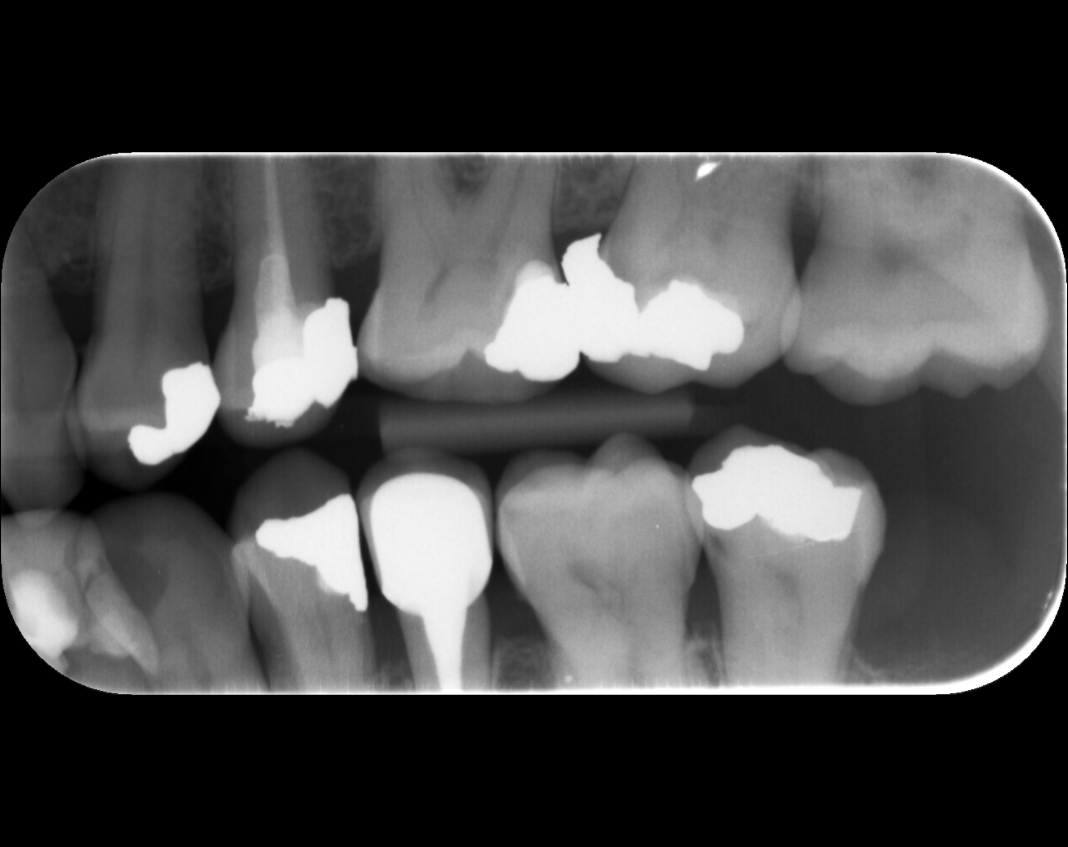
\includegraphics[width=\linewidth]{images/bitewing_xray.png}}\;
        \ffigbox[\FBwidth]{\caption{Periapical X-ray image, source \cite{Creanga2015}}\label{fig:periapical_sample}}%
        {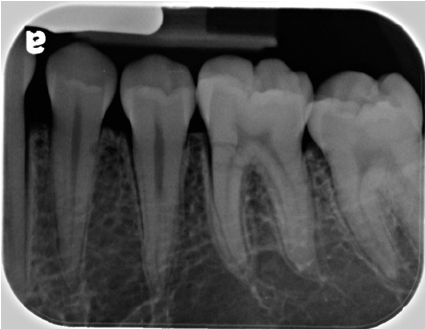
\includegraphics[width=\linewidth]{images/periapical_xray.png}}
    \end{floatrow}
\end{figure}

\subsubsection{Classification of dental caries from bitewing X-ray}
\label{sec:caries_classification}
Dental caries are classified on multiple bases. The common ones are the depth of the lesion or lesion activity. \newline
A frequently used classification scheme associated with bitewing radiographs was proposed by Pitts \& Fyffe in 1988 \cite{2019a}, including a total of 4 categories, three for cavitated lesions and one for non-cavitated lesions.
\begin{itemize}
    \item \textbf{D0} Surface sound. No evidence of either treated or untreated caries.
    \item \textbf{D1} Initial Caries. No detectable loss of tooth substance. Staining in fissures or rough spots in enamel may be visible, but these spots do not catch the explorer.
    \item \textbf{D2} Enamel caries. Demonstrable loss of tooth substance. The chalky or crumbled texture of the material within the cavity. No evidence that cavitation has penetrated through the enamel layer into the dentin.
    \item \textbf{D3} Caries of dentin. The floor or wall of the cavity is softened. The tip of the explorer must enter a lesion with certainty.
    \item \textbf{D4} Pulpal involvement. Deep cavity with probable involvement of the pulp. A probe should not be used to probe the pulp.
\end{itemize}

\subsubsection{Periapical X-ray}
Periapical X-ray portrays the tooth from the crown to where the root attaches to the jaw; hence, the whole tooth length is visible. As illustrated in Figure \ref{fig:periapical_sample}, it only shows the upper or lower teeth in one part of the jaw.  Periapical X-ray detects any abnormalities in the root and any periapical lesions.

\subsubsection{Panoramic X-ray}
This extraoral dental image shows the entire mouth area, including the upper and lower jaw and adjacent structures. It depicts the full dentition, including teeth that have not erupted yet. Impacted teeth, i.e. wisdom teeth as seen in Figure \ref{fig:panoramatic_xray}, can be identified as well. Panoramic X-ray is often used before major procedures or to diagnose jaw tumors, cysts, fractures, or sinusitis. Nevertheless, it is not usually taken to diagnose dental caries \cite{clevland_xray}.

\begin{figure}
    \centering
    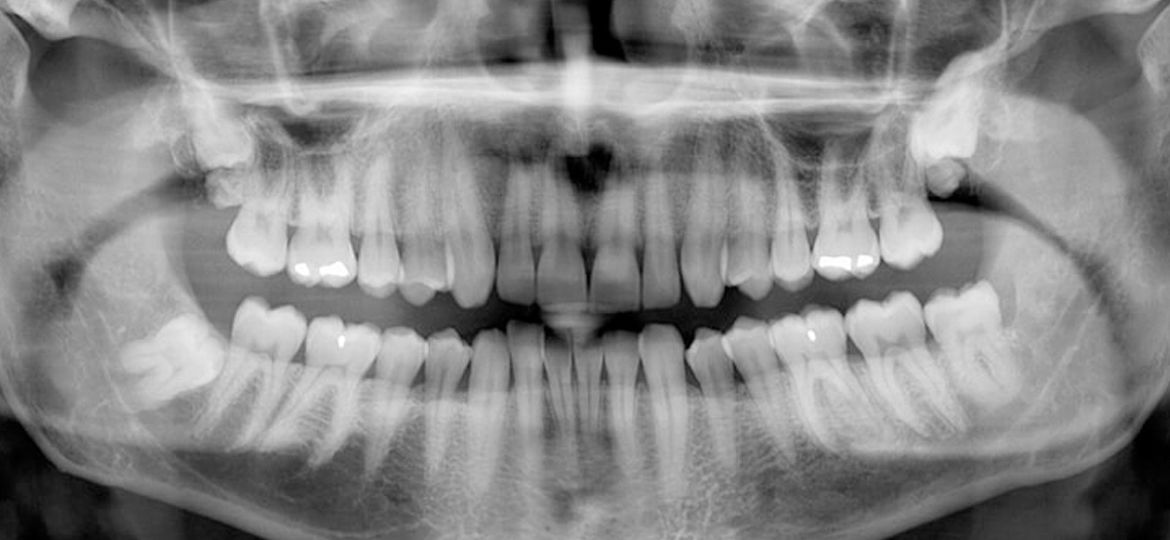
\includegraphics[width=\linewidth]{images/panoramatic_xray.jpg}
    \caption{Panoramic X-ray image, source \cite{Panoramatic2017}}
    \label{fig:panoramatic_xray}
\end{figure}


\subsubsection{Digital imaging fiber-optic transillumination (DIFOTI)}
DIFOTI is different from the previously mentioned types of dental imaging. It works with infrared fiber-optic light and not an X-ray, unlike the others. A lesion's optical properties differ from those in healthy dental tissue, making it appear darker. DIFOTI enables the detection of fissure/occlusal caries, interproximal caries, and fractures and cracks in the tooth. It is a noninvasive method since it does not expose the patient to ionizing radiation \cite{Strassler2014}.

\subsection{Treatment}
Treatment is suggested based on the progression of the lesion and the patient's risk profile. In some cases, only instructions to increase oral hygiene together with fluoride toothpaste are enough to stop the progression and lead to remineralization of the enamel. The dentist can suggest an application of a sealant to prevent further progression of the lesion. If this treatment is perceived as insufficient or if the carious lesion is already cavitated, restoring the tooth is required. This consists of removing all dental decay and filling the cavity with restorative material such as dental composite or amalgam \cite{2019a}\cite{2015}.

\chapter{Theoretical background}
\label{chapter:theoretical_bg}
\section{Computer vision tasks}
\begin{figure}
    \centering
    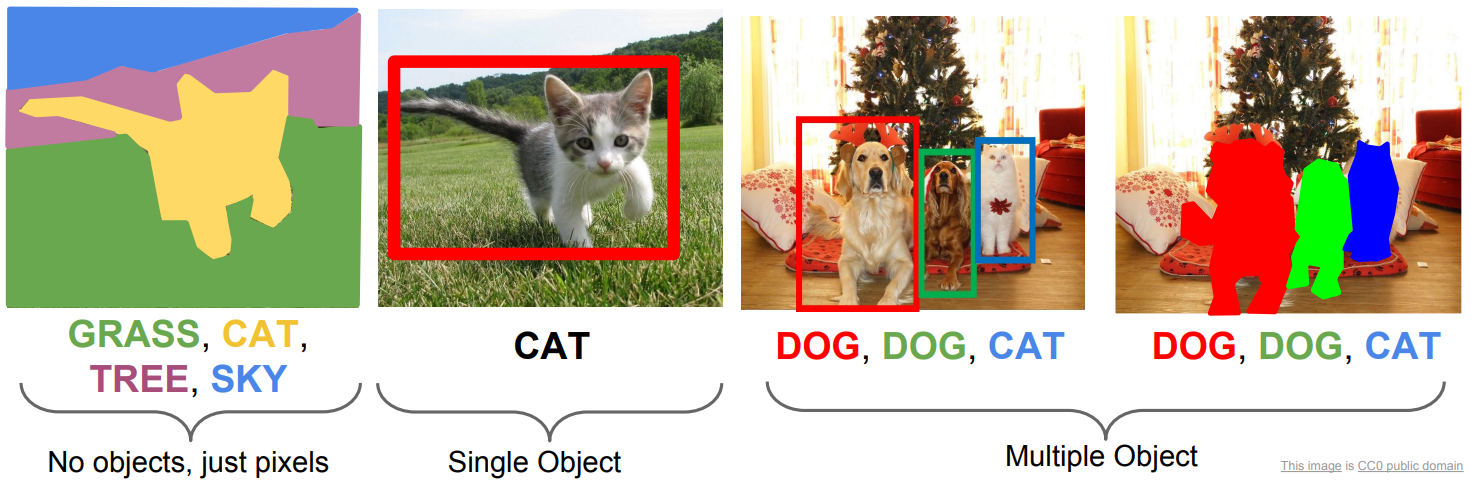
\includegraphics[width=\linewidth]{images/computer_vision_tasks.png}
    \caption{From the left: semantic segmentation, object localization, object detection, instance segmentation}.
    \label{fig:computer_vision_tasks}
\end{figure}
This section provides a brief overview of standard computer vision tasks.
\subsection{Classification}
Let's say we have an image $\mathbf{x}$. In a classification task, our goal is to assign one of $n$ possible classes to the image:
\begin{align}
    \hat{y} = f_\theta\left(\mathbf{x} \right),
\end{align}
where $f$ is a mapping, sometimes called a model, and $\theta$  represents model parameters if it holds that $\hat{y}=y$, where $y$ is a true class of the image $\mathbf{x}$, the classification is considered to be correct.
It is possible to output $\mathbf{p} \in \mathbb{R}^n$ instead of $\hat{y}$, where $p_i \in \mathbf{p}$ is probability of $i = y$, modeled by $f_\theta$.

\subsection{Semantic segmentation}
For an input image $x \in \mathbb{R}^{n \times m}$, the goal is to output $\mathbf{\hat{Y}} \in \mathbb{R}^{n \times m}$, where $\hat{y_{i,j}}$ is the predicted class of pixel $i,j$ in image $\mathbf{x}$. Similarly to the classification problem, we can output matrix $\mathbf{P} \in \mathbb{R}^{n \times m \times c}$, where $p_{i,j,c}$ is the probability of $pixel_{i,j}$ belonging to class $c$. A sample of semantic segmentation output can be seen in Figure \ref{fig:computer_vision_tasks}.

\subsection{Object detection}
\label{subsec:object_detection}
In object detection, the goal is to locate and recognize objects of interest in image $\mathbf{x}$. A rectangle and a category represent a ground truth object. Model predicts $\mathbf{Y} \in \mathbb{R}^{n \times 6}$ values for each image. Each row of $\mathbf{Y}$ consists of four numbers, which describe a rectangle, the category of the object inside the rectangle, and a number in the range from 0 to 1 called the confidence. In literature, we can see the term score instead of confidence. Nevertheless, the meaning remains the same: Certainty of the network regarding the particular prediction described by the bounding box and category. Please note that the confidence of predictions does not sum to one. In other words, we are not talking about probabilities since multiple detections per image can correspond to the ground truth.

\subsection{Instance segmentation}
Instance segmentation is similar to semantic segmentation, with the alteration saying that two objects of the same category would have different ground truth values. If we have $\mathcal{O}_1, \mathcal{O}_2$, where $\mathcal{O}_i \subset \mathbf{x}$ are pixels of object $i$ in image $\mathbf{x}$. Then
\begin{align}
    o_{1_i} \neq o_{2_i} \quad \text{for} \quad o_{1_i} \in \mathcal{O}_1, o_{2_i} \in \mathcal{O}_2;\forall i.
\end{align}

\section{Data format in object detection}
As described in Section \ref{subsec:object_detection}, the position of an object is denoted by a bounding box.  The four parameters used to describe a bounding box can be selected in multiple ways. This ambiguity led to a disjoint notation. The most widespread are as follows.
\subsection{PASCAL VOC}
The format was introduced together with the PASCAL VOC dataset, the most popular dataset for object detection algorithm benchmarking in 2010. The bounding box is described by points $p_1(x,y),p_2(x,y)$ located in the top-left and bottom right corner. The coordinates range from 0 to image width/height in pixels. All the annotations are stored in a single XML file \cite{Everingham2009,Padilla2021}.
\subsection{COCO}
COCO data format is represented by a single JSON file containing all bounding boxes of the dataset. The boxes are described by the top-left corner point $p(x,y)$ and the width and height of the box. The coordinates and box dimensions are again in the range 0 to image dimensions. In MS COCO, the annotation can be accompanied by a piece of additional information to solve the task as an instance segmentation problem.
\subsection{YOLO}
This format was introduced together with the first YOLO architecture \cite{Redmon2015}, and this annotation style is still persistent whenever working with the YOLO-family neural networks.
In this format, the annotations are divided into multiple TXT files and each of them contains annotations for a single image.
The bounding box is described similarly as in the COCO dataset, but the coordinates are normalized to be in the 0 to 1 range. The advantage of this approach is that the annotations do not have to be modified when image dimensions are scaled \cite{Redmon2015, Padilla2021}.


\section{Metrics}
\subsection{Intersection over union (IOU) }
Intersection over union, also known as the Jaccard index, is defined as demonstrated: Let $B_{gt}$ and $B_p$ be a ground truth and a predicted bounding box. The Jaccard index $J$ is calculated as
\begin{align}
    IOU = J(B_p, B_{gt}) = \frac{area(B_p \bigcap B_{gt})}{area(B_p \bigcup B_{gt})}.
    \label{eq:iou}
\end{align}
From the Equation \ref{eq:iou}, we can observe that the lowest value of IOU is 0. This means there is no overlap and the maximal value is 1, indicating a perfect match.
We use a predefined threshold value of IOU to decide if the predicted bounding box matches the ground truth. Usually, we choose this threshold to be 0.5 or above.

IOU can be defined for the semantic segmentation task with two classes (e.g. background and target class). Let $\mathbb{\hat{Y}} \in \mathbb{R}^{m \times n}$ be the mask of the predicted values, where $\hat{y}_{i,j} = 1$ if the model predicts, that pixel $i,j$ belongs to target class. The IOU is defined as:
\begin{align}
    IOU = \frac{\sum_{i=1}^{m} \sum_{j=1}^{n} \hat{y}_{i,j} \wedge  y_{i,j}}{\sum_{i=1}^{m} \sum_{j=1}^{n} \hat{y}_{i,j} \vee  y_{i,j}},
\end{align}
where $y_{i,j} \in \mathbf{Y} \in \mathbb{R} ^ {m \ times n}$ is the ground truth value for pixel $i,j$.


\begin{figure}
    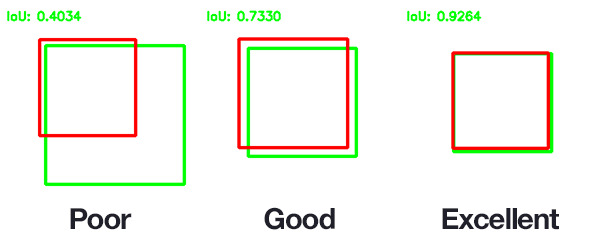
\includegraphics[width = 0.9\linewidth]{images/IOU.jpg}
    \caption{Examples of IOUs for different overlaps between GT and predicted box, source. \cite{Cowton2019}}
    \label{fig:iou}
\end{figure}

\subsection{Precision and recall}
\subsubsection{Precision}
\label{subsec:precision}
When speaking about object detection, we say that a prediction is a true positive (TP) if the IOU value is greater than the predefined threshold $\tau$. If otherwise, the prediction is treated as a false positive (FP). Let's assume there are N predictions of our model, from which S are correct. Precision is defined as
\begin{align}
    Precision(\tau, \gamma) = \frac{TP(\tau, \gamma)}{TP(\tau, \gamma) + FP(\tau, \gamma)},
\end{align}
where $\gamma$ is the confidence threshold, meaning we discard all predictions with confidence smaller than $\gamma$. Note that for fixed value of $\tau$ are $FP(\gamma)$ and $TP(\gamma)$ decreasing functions of $\gamma$ \cite{Padilla2021}.

\

\subsubsection{Recall}
\label{subsec:recall}
If there is a ground truth bounding box for which there are no given detection values of $\gamma$ and $\tau$, we say it is a false negative (FN). If we consider a dataset with G ground-truths and N predictions of which S is correct, where $(S \leq G)$, the recall is expressed as:
\begin{align}
    Recall(\tau, \gamma) = \frac{TP(\tau, \gamma)}{ TP(\tau, \gamma) + FN(\tau, \gamma)}.
    \label{eq:recall}
\end{align}
Since the value of $FN(\gamma)$ increases with the growing value of $\gamma$, we see that recall is the decreasing function of $\gamma$.

\subsubsection{F1 score}
The value of the F1 score is computed as the harmonic mean of precision and recall.
\begin{align}
    F1(\tau, \gamma) = \frac{2 \cdot Recall(\tau,\gamma) \cdot Precision(\tau, \gamma)}{Recall(\tau,\gamma) + Precision(\tau, \gamma)}.
\end{align}

\subsubsection{Precision-recall curve (PR curve)}
From Subsections \ref{subsec:precision} and \ref{subsec:recall}, we were able to observe that precision mainly grows as we increase the confidence threshold $\gamma$, while at the same time recall decreases. The precision-recall curve captures the relation between precision and recall. An example of the curve is illustrated as the blue line in Figure \ref{fig:pr_curve}. In other words, we can say that the precision-recall curve is a mapping
\begin{align}
    \gamma \rightarrow Precision(\gamma) \times  Recall(\gamma),
    \label{eq:pr_curve}
\end{align}
where $\gamma$ ranges from 1 to 0.

\subsubsection{Mean average precision (mAP)}
To calculate mAP we first need to get the PR-curve and then interpolate the precision values. Suppose that we have $K$ different confidence values $\gamma$ among model predictions, which are ordered as
\begin{align}
    \gamma(k),\: k = 1,2,...,K,  \; \text{such that } \gamma(i) > \gamma(j) \: for \: i > j.
\end{align}
The interpolated precision-recall curve is then defined as
\begin{align}
    Precision_{interp}(R) = \max_{k|Recall(\gamma(k)) \geq R} \{  Precision(\gamma(k)) \},
\end{align}
where $R$ is a real value contained in interval [0,1] \cite{Padilla2021}.
The interpolated precision-recall curve is pictured in Figure \ref{fig:pr_curve} in red color. Now, we can compute the average precision (AP) as the area under the interpolated PR curve.
In practice, there are two different ways to approach the Reimann integral. They differ in the number of samples used to compute the integral and are called N-point and all-point interpolation. The N-point, specifically 101 point interpolation, is used in the MS COCO competition. On the other hand, the all-point interpolation is nowadays used in PASCAL VOC challenges \cite{Padilla2020, Padilla2020}.

Since the AP is calculated per class, the mean average precision is defined as the average in all categories.

In Subsections \ref{subsec:precision} and \ref{subsec:recall}, we stated that precision and recall depend on a predefined IOU threshold $\tau$ to consider prediction as true positive. This dependency makes the value of MAP vary over different values of $\tau$. The threshold value used for computation of the mAP is usually denoted in the metrics name, such as $AP@.5$ in the case of MS COCO. \footnote{Note that even though the mean average precision is computed, the $AP$ shortcut, which stands for average precision, is used.} The standalone $AP$ without any numerical values attached to it usually refers to the official COCO metric. The official COCO metric is in its explicit form written as $AP@[.5:0.05:0.95]$ and is computed as the average of MAP values for ten different $\tau$ values, ranging from 0.5 to 0.95.

The letters S, M,  and L in the subscript, such as $AP_S$ denote that the metrics are calculated for a subset of ground truth predictions only. Taking into the consideration only bounding boxes with area $\leq 32^2$ pixels, $32^2 \le $ area $ \leq 96^2$ pixels and area $> 96^2$ pixels

\subsection{Mean average recall in MS-COCO (mAR)}
PyCOCOtools, the official metrics for MS-COCO benchmark \cite{pycocotools}, compute the average recall (AR) by the following approach: Predictions are sorted according to their confidence in a decreasing order. We take $n$ boxes with the highest confidence values and evaluate their recall by Equation \ref{eq:recall} for a predefined IOU threshold $\theta$. We use a similar notation as in the case of AP, where $AR@.X_{na}$ denotes the average recall computed for IOU threhsold $X$, where we consider $n$ most confident predictions. By $a \in \{ S, M, L, \text{all} \}$ we denote size of the rectangles, for which AR is computed. If we omit some of those, the following default values are used $a=\text{all}, n = 100, X = [.5:0.05:0.95]$.

\begin{figure}
    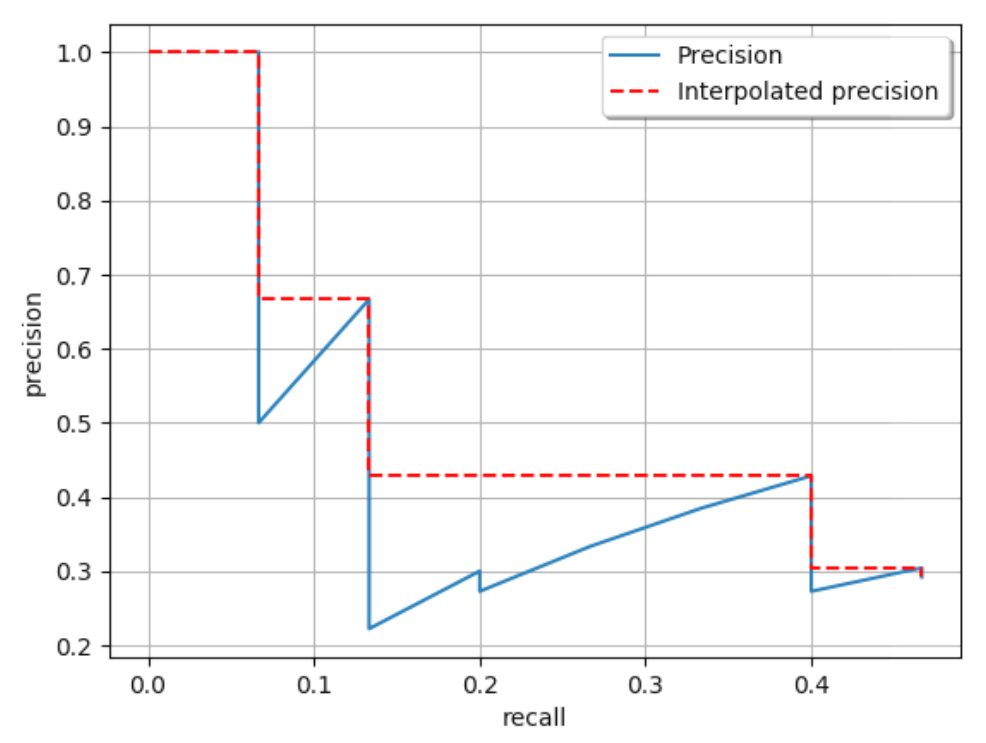
\includegraphics[width = 0.78\linewidth]{images/PR-curve.png}
    \caption{Standard and interpolated precision-recall curve, source \cite{Padilla2020}}
    \label{fig:pr_curve}
\end{figure}


\subsubsection{Cross-Entropy loss}
\label{sec:cross_entropy}
Let $\mathbf{y} \in \mathbb{R}^n, y_i \in \{ 0, 1 \}$ be a vector of ground truth classes and $\hat{\mathbf{y}} \in \mathbb{R}^n$ be a vector of model preditions, where $\hat{y_i} \in [0, 1]$ is the predicted probability, that $i_{th}$ element belongs to class $1$. The cross-entropy loss is computed as follows \cite{Jadon2020}:
\begin{align}
    L_{CE}(\mathbf{y}, \hat{\mathbf{y}}) = - \frac{1}{N} \sum_{i=1}^N y_i \log (p(\hat{y_i})) + (1 - y_i) \log (1 - \hat{y_i})
\end{align}

\subsubsection{Soft Dice Loss}
Let's consider $\mathbf{y}$ and $\hat{\mathbf{y}}$ as in section \ref{sec:cross_entropy}, Soft Dice Loss is then computed as:
\begin{align}
    SDL(\mathbf{y}, \hat{\mathbf{y}}) = 1 - \frac{\sum_{i=1}^N 2y_i \hat{y_i}}{\sum_{i=1}^N y_i + \sum_{i=1}^N \hat{y_i}}
\end{align}
Dice Loss is computed in the same way, we only threshold values of $\hat{\mathbf{y}}$ prior to computation of the loss \cite{Softdiceloss,Jadon2020}.

\section{Optimization}
In deep learning, a defined loss function that should be minimized usually does not have an analytical solution, or the solution cannot be evaluated for computational reasons. Therefore, the iterative numerical optimization approach is used, where we compute the gradient of the loss function with respect to the parameters of the optimized model. Those are updated by changing their values in the negative direction of the computed gradient.
\subsection{Optimizers}
The most simple optimizer is Stochastic Gradient Descent (SGD), which in each step updates the weights by stepping in the opposite direction of the gradient The learning rate affects the length of the step.

Many advanced optimizers that increase the speed of convergence are available. Commonly used are SGD with moentum, Adam and AdamW.

\subsection{Weight decay}
We can add the $L_2$ of the model weights to the loss function. This term is called weight decay and should decrease the discrepancy between performance on training and testing part of the dataset.

\subsection{Learning rate schedulers}
Learning rate is considered to be one of the most, if not the most important parameter, in deep learning. It is usually beneficial to change the learning rate during the course of training. This can be done manually or automated by an algorithm that increases or decreases the learning rate based on the set of predefined rules. This algorithm is called the learning rate scheduler.
\begin{figure}
    \centering
    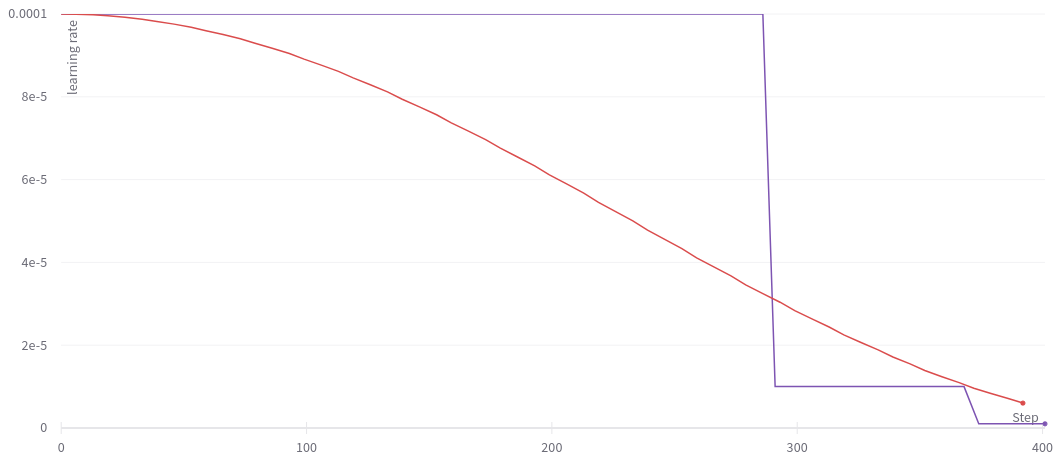
\includegraphics[width=0.5\linewidth]{images/schedulers.png}
    \caption{Learning rate schedulers: Cosine annealing is red, Reduce learning rate on plateau has purple color}
    \label{fig:schedulers}
\end{figure}

\subsubsection{ReduceLROnPlateau}
We couple the scheduler with a model metric, and when the improvement of the metric stalls for a predefined period, the learning rate decreases.
The scheduler is not heavily reliant on the setting of its hyperparameters, making it a go-to starting choice for most developers.

\subsubsection{Cosine annealing}
Cosine annealing changes the value of learning rate according to the equation \ref{eq:cosine_annealing}, where $T$ is half-period of the cosine.
\begin{align}
    lr(t) = lr_{min} + \frac{1}{2} \left( lr_{max} - lr_{min} \right) \left( 1 + \cos \left( \frac{t}{T}\pi \right) \right)
    \label{eq:cosine_annealing}
\end{align}
It is commonly used with two different settings. Either we set $T$ to estimated length of the training. The learning rate than decreases throghout the training, as can be seen in Figure \ref{fig:schedulers}, or we select small value of $T$ and the learning rate oscilates in predefined boundaries multiple times throughout the training. This should help the optimizer to overcome saddle points.

\section{Artificial neural network (ANN)}
The mechanisms of the human brain inspire artificial neural networks. Human neuron cells are in ANN replaced by artificial neurons, which are defined as:
\begin{align}
    y = f \left( \boldsymbol{w}^T \boldsymbol{x}  + b \right).
\end{align}
Where $\boldsymbol{x}$ is a vector of inputs, $\boldsymbol{w}$ stands for weights and $b$ is bias. Symbol $f$ denotes an activation function f : $\mathbb{R} \rightarrow \mathbb{R}$. The artificial neuron proposed by Frank Rosenblatt in the perceptron algorithm worked with a step function \cite{Rosenblatt1958}, but nowadays, different functions such as ReLu, sigmoid or tanh are used. The output of the neuron $y$ is called activation of the neuron.

Neurons are usually structured into layers. The connection between layers depends upon the architectural choice. First ANNs used fully connected layers, meaning that the input into a neuron in layer $n$ was composed of all activations from layer $n-1$. Fully connected neural networks are nowadays sparsely used in computer vision. Convolutional neural networks (CNNs) or vision transformers are used instead. In the case of CNNs we limit neurons' receptive field to the local neighborhood only; this decreases the computation complexity and includes our prior knowledge of pixel neighborhood in the input image. Having the same weights for the whole input makes the network invariant to shifts in the input.

\subsection{Convolutional layer}
A convolutional layer consists of $C_{out}$ neurons, each having $C_{in}, H, W$ receptive field. Those neurons are called kernels with width $W$ height $H$ and several input channels $C_{in}$. In each layer, we convolve\footnote{Even though we usually refer to convolution, in practice, cross-correlation is used instead. Terms cross-correlation and convolution are used interchangeably.} the input $X$  with the kernel $W$, the output $Y$ is defined by:
\begin{align}
    y_{o,i,j} = \sum_{c_{in}} \sum_{\Delta i} \sum_{\Delta j} x_{c, i+\Delta i, j + \Delta j}  w_{o,c, \Delta i, \Delta j}
\end{align}
Nowadays, modifications of convolutional layers are proposed, such as dilated convolution, grouped convolution, or depth-wise separable convolutions are used. However, the fundamentals remain the same: Filter sliding over the input produces an output.

\begin{figure}
    \centering
    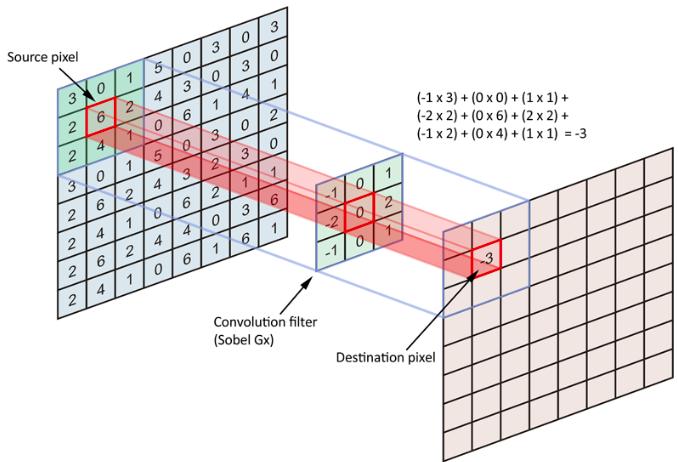
\includegraphics[width=0.9\linewidth]{images/conv_img.png}
\end{figure}

\subsection{Activation functions}
A non-linear activation function usually follows the output of the convolutional layer. Many activation functions are at our disposal, but the most commonly used is ReLU and its derivatives, such as SERLU, SELU, ELU, Swish, and Leaky ReLU. Values of those functions are depicted in Figure \ref{fig:activation_functions}.

\subsection{Normalization layers}
\label{sec:normalization_layers}
Normalization layers make the training of ANNs faster and more stable. It has been shown, that normalization-layers decrease the generalization gap ,while increasing the convergence speed \cite{Ioffe2015,Wu2018}. The normalization layers differ in spatial axis, across which, the normalization statistics is computed, this is illustrated in Figure
\subsubsection{Batch-normalization}
The most normalization layer is batch normalization, which computes the output of the layer $y_i$ as:
\begin{align}
    \hat{x_i} \leftarrow \frac{x_i - \mu_{\mathcal{B}}}{\sqrt{ \sigma _{\mathcal{B}^2} + \epsilon}}; \qquad y_i \leftarrow \gamma \hat{x_i} + \beta
\end{align}
where $\gamma$ and $\beta$ are learnable parameters, $\mathcal{B}$ denotes, that this value is computed over a mini-batch.


\subsubsection{Group-normalization}
\label{sec:group_norm}
Wu et al. \cite{Wu2018} proposed a normalization method, where the statistics are computed over groups of channels. We et al. showed that group normalization outperforms batch normalization when both layers are used with batch sizes smaller than eight.

The disadvantage of group normalization is the introduction of a new group size $G$ hyper-parameter, which needs to be tuned to obtain the results claimed by the authors \cite{Wu2018}.

\begin{figure}
    \begin{floatrow}[2]
        \ffigbox[0.9\FBwidth]{\caption{Graphs of ReLU based activation functions, source \cite{Zhang2018}}\label{fig:activation_functions}}%
        {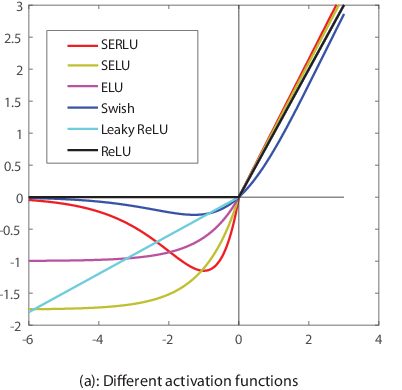
\includegraphics[width=\linewidth]{images/activation_functions.png}}\quad
        \ffigbox[1.1\FBwidth]{\caption{Batch and group normalization layers with denoted axes, across, which the normalization statistics is computed}\label{fig:normalization_layers}}%
        {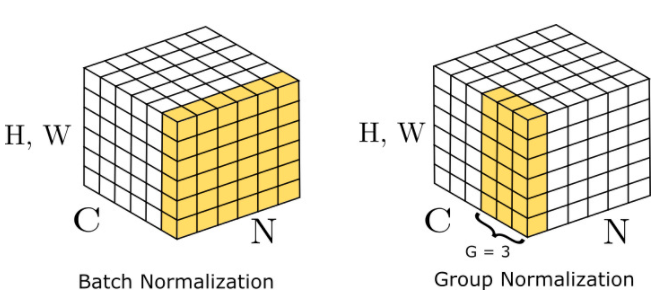
\includegraphics[width=\linewidth]{images/group_batch_norm.png}}
    \end{floatrow}
\end{figure}



\section{Transformer architecture}
Transformer architecture debuted in computer vision in 2021 and has achieved outstanding results, beating state-of-the-art models in multiple benchmarks across all computer vision tasks. As of May 2022, the best-performing models in the main computer vision benchmarks are based on transformer architecture. We think of the following benchmarks to be the main ones in computer vision:  ImageNet benchmark (classification task), COCO (object detection), ADE20K (semantic segmentation).

The transformer architecture was proposed already in 2017 for the task of natural language processing (NLP). We will briefly introduce transformer architecture for the NLP task since it is crucial for understanding transformers for computer vision.

\subsubsection{Transformers in NLP}
Transformer architecture was introduced in the paper Attention is all you need \cite{Vaswani2017} for NLP. NLP is a task where input is a sequence of words of length $n$ and output is a sequence of $m$ words, where $n$ and $m$ usually differ. The sequence of words is converted into a sequence of vectors. There are multiple options for how to embed words into the vector. Commonly used is TD-IDF or Word2Vec\cite{Li2018}. Positional encoding is added to those vectors are then the encoder block processes it. The novel key component is the self-attention module, where for the input sequence of vector values $V$, keys $K$ and queries $Q$ are computed. We output values and keys from the encoder, and from the decoder's self-attention module, we output queries. We then take keys and values from the encoder and queries from the decoder and input them into another attention block:
\begin{align}
    Attention \left(Q,K,V \right) = \text{softmax} \left( \frac{QK^T}{\sqrt{d_k}} \right)V,
\end{align}
where $d_k$ is dimension of keys. More details can be seen in Figure \ref{fig:nlp_transformer} or in \cite{Vaswani2017}.

\begin{figure}
    \centering
    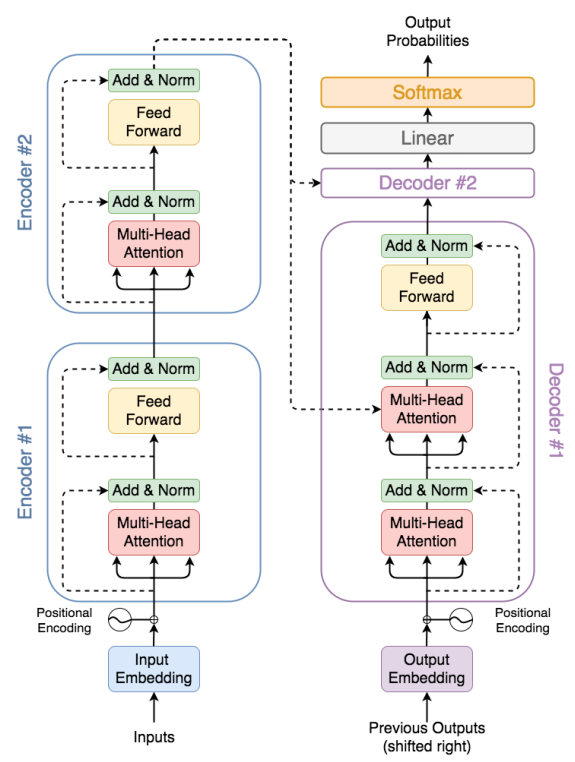
\includegraphics[width=0.5\linewidth]{images/two_layer_transformer.png}
    \caption{Architecture of transformer with two encoders and two decoders, source \cite{Yin2020}}
    \label{fig:nlp_transformer}
\end{figure}

\subsection{Transformers in computer vision}
The first transformer-based model was the Vision Transformer (ViT) which is capable of image classification only. It is composed of multiple encoder blocks stacked on top of each other; those blocks are the same as those used by the transformer for the NLP task. On the top encoder block is attached a multi-layer perceptron (MLP) head, which outputs values for each class. Those can be converted into corresponding probabilities by a softmax layer. The input into ViT are $16 \times 16$ image patches linearly projected into vectors; the whole architecture is shown in Figure
\begin{figure}
    \centering
    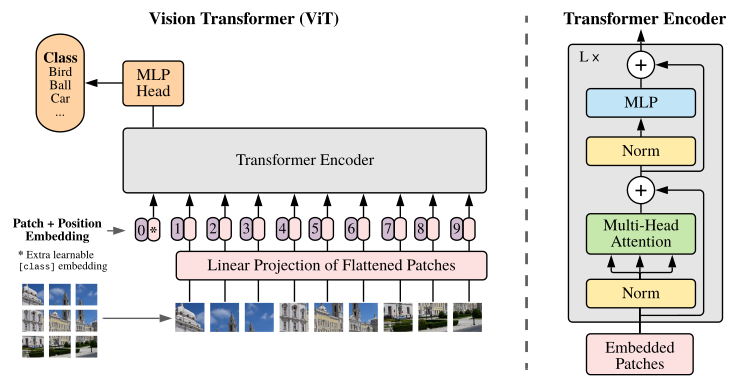
\includegraphics[width=\linewidth]{images/vision_transformer.png}
    \caption{Architecture of ViT, source \cite{Dosovitskiy2020}}
    \label{fig:vision_transformer}
\end{figure}


\section{General architecture for object detection}
Even though there is a wide variety of architectures for object detection, the core principles remain the same. The model is composed of three main parts: backbone, neck, and head, as depicted in Figure \ref{fig:object_detection_architecture}. Each of those blocks can usually be swapped for a different one, fulfilling the same purpose. This gives us great flexibility and allows us to try different combinations of those blocks.



\subsubsection{Backbone}
The purpose of backbones is to transform the input image into feature maps. For this purpose, we use classification models with the classification head removed. Most parameters of object detection models are usually part of the backbone. The extraction of useful feature maps is vital for other blocks to perform well. The most common backbones are models from the ResNet family.

\subsubsection{Neck}
The neck is responsible for the merging of features from the backbone. This is not a straightforward task since we usually use features from different backbone layers. This allows us to get semantically strong features from deeper layers and more detailed information from earlier ones. Common neck architectures are feature pyramid network or PANet \cite{Lin_2017_CVPR}.
\begin{figure}
    \centering
    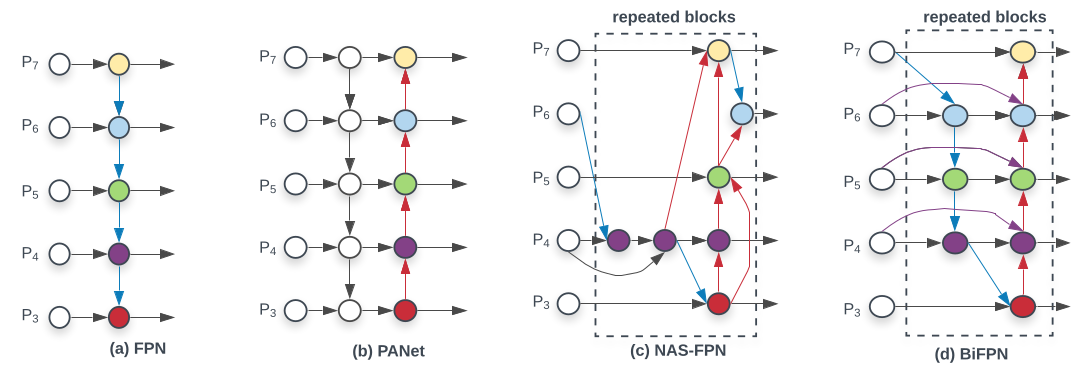
\includegraphics[width=\linewidth]{images/necks_architecture.png}
    \caption{Architecture of different necks for feature fusion, source \cite{Tan2019}}
    \label{fig:necks}
\end{figure}

\subsubsection{Head}
The head is responsible for predicting the position of boxes and their classification. It uses the features extracted by the backbone and merged by the neck. Based on the approach to box prediction, we differ them into Dense prediction heads (YOLO, RetinaNet) or Sparse prediction heads(Faster R-CNN) \cite{Bochkovskiy2020}.


\begin{figure}
    \begin{floatrow}[2]
        \ffigbox[\FBwidth]{\caption{The schema of two-stage detection process of Faster R-CNN }\label{fig:faster_rcnn}}%
        {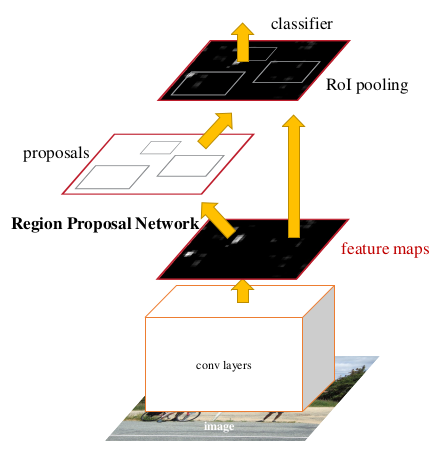
\includegraphics[width=\linewidth]{images/FasterRcnn.png}}\qquad
        \ffigbox[\FBwidth]{\caption{General architecture for object detection, source \cite{Chen2019}}\label{fig:object_detection_architecture}}%
        {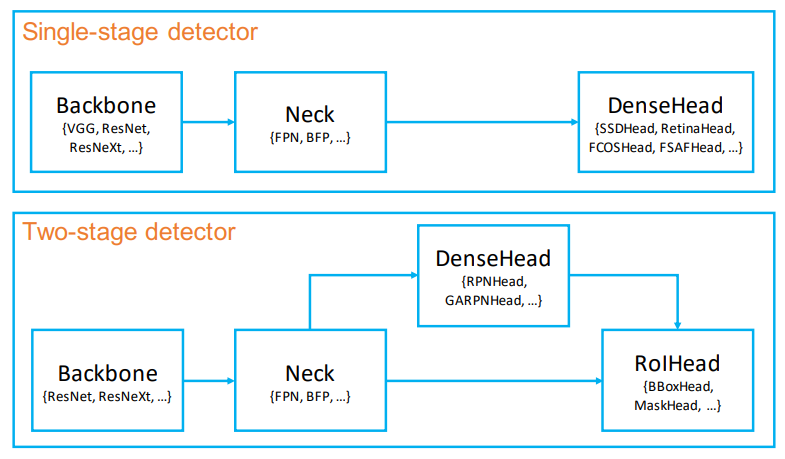
\includegraphics[width=\linewidth]{images/object_detection_architecture.png}}
    \end{floatrow}
\end{figure}

\section{Backbone models}
This section will introduce multiple architectures of neural networks, which were used as a backbone throughout our work.
\subsection{ResNet}
ResNet architecture was introduced by He et al. \cite{He2015} and proposed a novel element of deep-learning architectures - an identity shortcut connection sometimes called a skip-connection. Let $\mathbf{x}$ be the input into a block composed of multiple convolutional layers with activation functions in between\footnote{Addition of batch-normalization, or other layers is possible}; we will call this block a mapping $\mathcal{F}$. The output of the residual block $\mathcal{H}$, derived from $\mathcal{F}$ is defined as:
\begin{align}
    \mathcal{H}\left(\mathbf{x}\right) = \mathcal{F} \left(\mathbf{x}\right) + \mathbf{x}.
\end{align}
The reasoning behind the residual block is to make it easier to learn the identity mapping if desired. This has other benefits, especially the improvement of the gradient flow during back-propagation, making it easier to optimize such blocks. This ease of optimization can be seen by inspecting the loss function landscape of a model with and without skip-connections in Figure \ref{fig:resnet_loss}.
Final ResNet architecture is composed of multiple residual blocks stacked one after another; the models vary in the number of layers used; this is denoted in the name with a number such as ResNet50 or ResNet101.

\begin{figure}
    \centering
    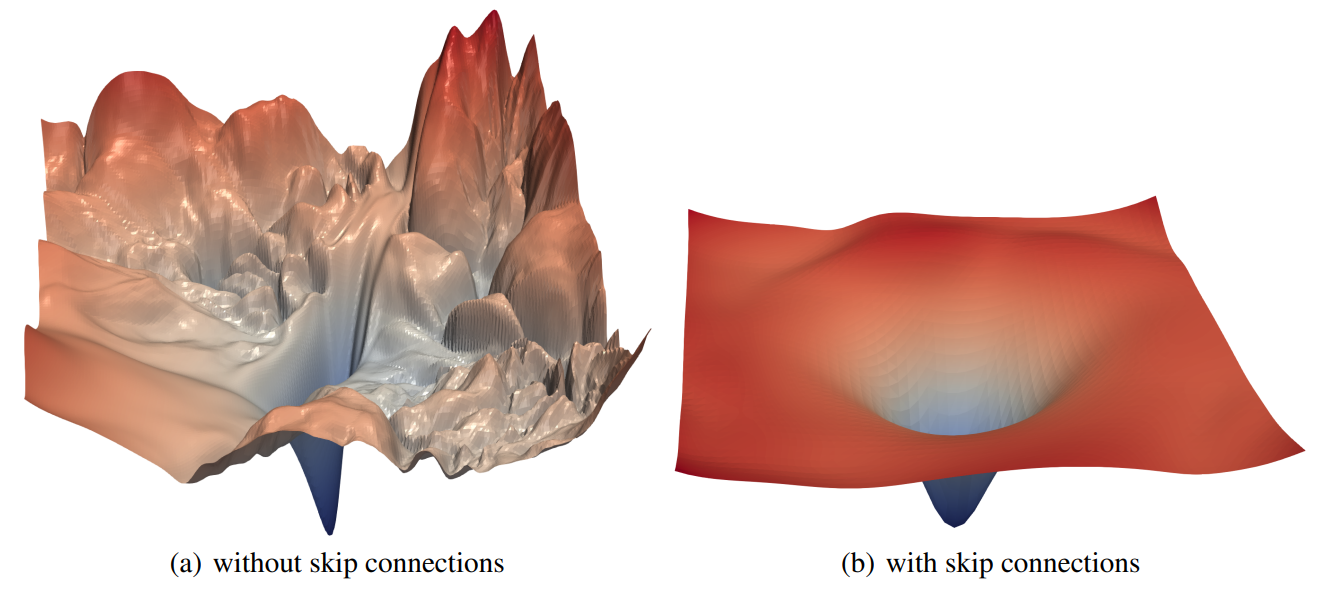
\includegraphics[width=\linewidth]{images/resnet_loss.png}
    \caption{Comparison of loss landscapes, source \cite{Li2017}}
    \label{fig:resnet_loss}
\end{figure}

\subsection{EfficientNet}
When scaling the model's size, we can increase: Number of layers (depth), the number of filters in each layer (width), or the width and height of feature maps (resolution). It has been a common practice to change only one of them. Tan and Le \cite{Tan2019a} did a multi-objective neural network search, where they tried to maximize objective function $O$ defined as:
\begin{align}
    O = ACC \left( m \right) \times \left[ FLOPS \left(m \right) / T \right] ^w,
\end{align}
where $ACC(m)$ and $FLOPS(m)$ are accuracy and floating-point operations (FLOPS) of model $m$, $T$ is the target number of FLOPS, and $w$ is a hyper-parameter controlling the trade-off between accuracy and number of FLOPS of the final model. This search resulted in the EfficientNet-B0 baseline model, which can be scaled to obtain a more extensive network called B1-B7.

\subsection{Swin transformer}
Swin transformer architecture overcomes the limitations of ViT, which is working with $16 \times 16$ image patches only. This is insufficient for segmentation and object detection tasks, where dense predictions are needed. Swin transformers are in the first layer working with $4 \times 4$ patches. Since the computation complexity of the self-attention layer grows quadratically with the number of input tokens, the authors overcome this by using neighbor patches only. Attention is thus computed with respect to tokens in the non-overlapping local window. As depicted in Figure\ref{fig:swin_pathces}, this local window for computing self-attention is shifted after every encoder layer. This shift introduces cross-window connections, which increase the modeling capacity of the model. After a particular number of encoder layers, neighbor patches are merged, which reduces the number of patches while increasing their size by a predefined factor. This mimics the behavior of CNNs, where we start with big, semantically weak feature maps and gradually decrease their dimensions while increasing their number. Having this kind of feature map allows using swin transformer as a general backbone for any task. \cite{Liu2021}

\begin{figure}
    \begin{floatrow}[2]
        \ffigbox[\FBwidth]{\caption{Hierachical structure of Swin Transformer compared with ViT, source \cite{Liu2021}}\label{fig:swin_hierarchy}}%
        {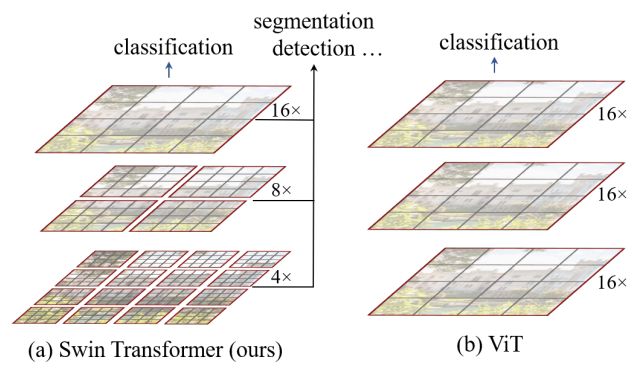
\includegraphics[width=\linewidth]{images/swint_transformer_hierarchy.png}}\qquad
        \ffigbox[\FBwidth]{\caption{Shift of local window for computation of self-attention, source \cite{Liu2021}}\label{fig:swin_pathces}}%
        {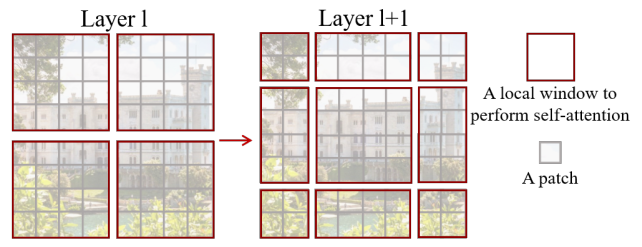
\includegraphics[width=\linewidth]{images/swint_transformer_patches.png}}
    \end{floatrow}
\end{figure}

\section{Detection models}
\label{sec:deteciton_models}

\subsection{Faster R-CNN}
Faster RCNN (Region-Based Neural Network) architecture is a two-stage detector. In the first stage, Region Proposal Network (RPN) finds regions of interest (ROI)and proposes bounding boxes corresponding to those regions. This is done by sliding a small neural network over the output of the backbone. In the second stage, features corresponding to positions of ROIs are extracted from the backbone and processed by a classification network, which decides if the region corresponds to a background or is one of the target classes. The schema of the architecture is in Figure \ref{fig:faster_rcnn}

\subsection{RetinaNet}
The biggest contribution of RetinaNet is the introduction of focal loss \cite{Lin2017}, see Figure \ref{fig:focal_loss}. It helps to mitigate to the problem if class imbalance by changing the formula Cross-Entropy loss. The penalization of well-classified samples decreases, increasing the importance of correct classification of hard-to-classify examples.

\begin{figure}
    \centering
    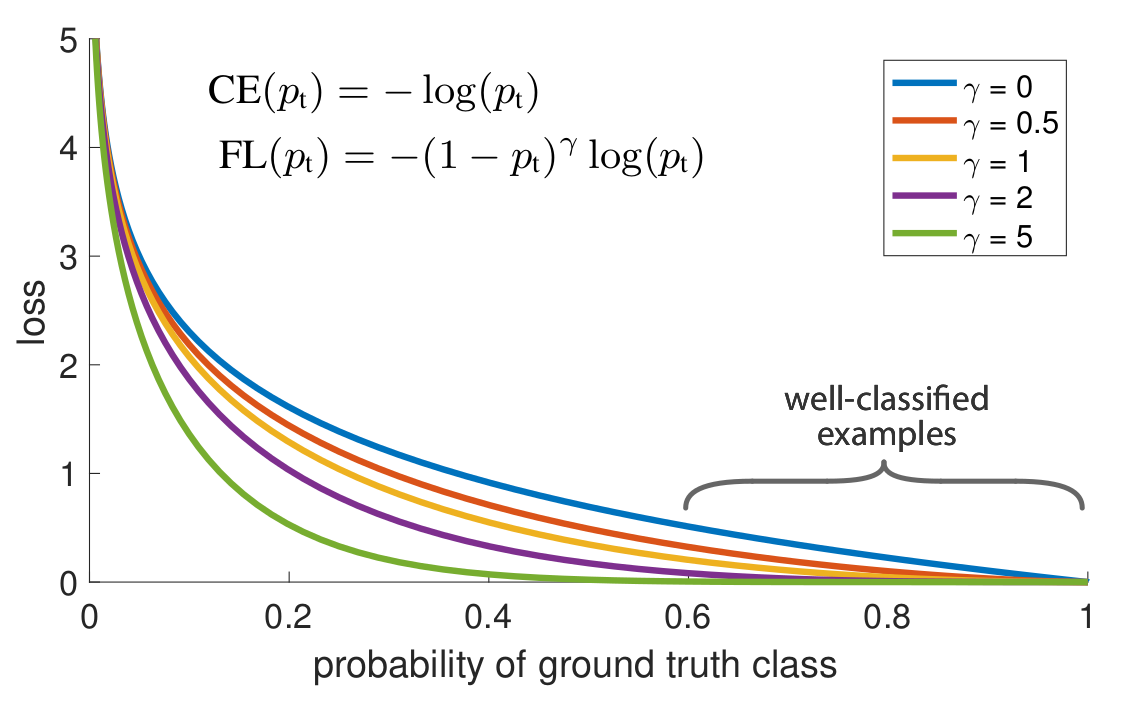
\includegraphics[width=0.7\linewidth]{images/focal_loss.png}
    \caption{Focal Loss, source \cite{Lin2017}}
    \label{fig:focal_loss}
\end{figure}


\subsection{EfficientDet}
EfficientDet tries to achieve a similar goal as EfficientNet: Propose a computationally effective architecture for object detection that would be scalable. Since an efficient backbone architecture was already proposed \cite{Tan2019a}, they focus mainly on feature fusion from multiple layers. Based on the study of FPN, PANet, and NAS-FPN, a Bidirectional feature pyramid network (BiFPN) was proposed as the most computationally effective neck architecture \cite{Tan2019}; it consists of multiple BiFPN blocks stacked on top of each other, see \ref{fig:necks}. The count of those blocks is dependent on the size of the used backbone.

\subsection{Models for image segmentation}
\subsubsection{U-Net}
\begin{figure}
    \centering
    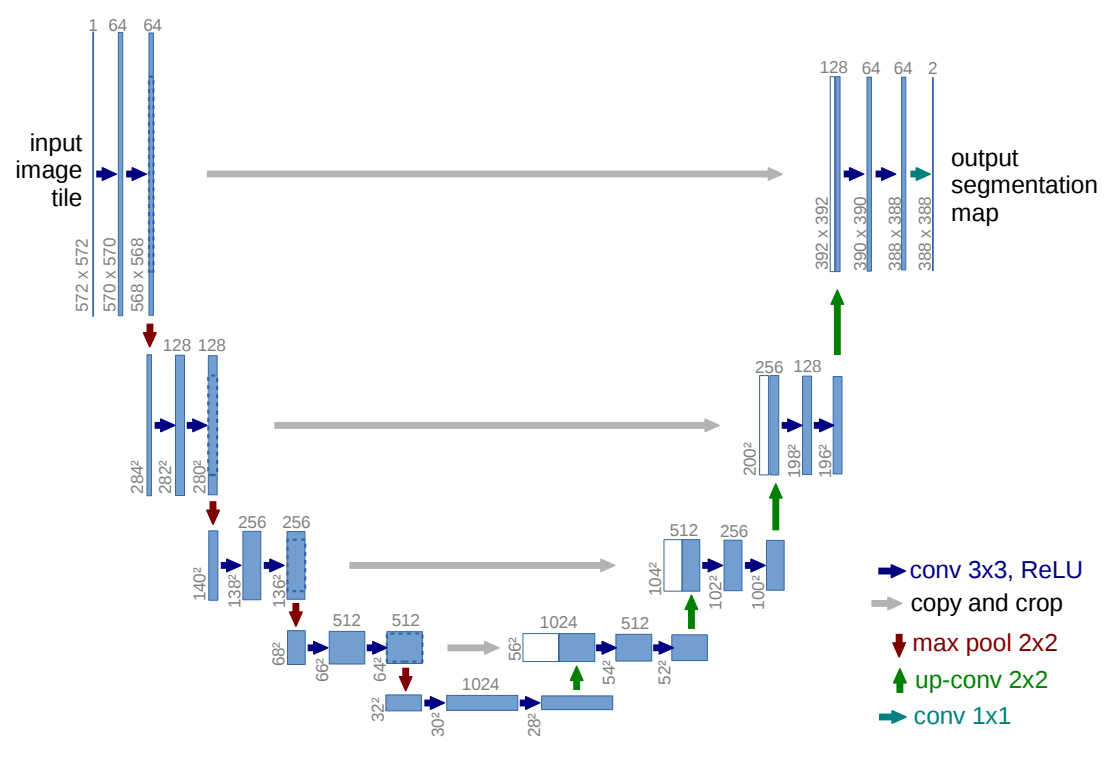
\includegraphics[width=\linewidth]{images/U-Net.png}
    \caption{Architecture of U-Net model, source \cite{Ronneberger2015}}
    \label{fig:unet_architecture}
\end{figure}
U-Net is an architecture for semantic segmentation, with an encoder-decoder structure as shown in Figure \ref{fig:unet_architecture}. The decoder extracts feature maps from the input image with an increasing semantical strength throughout the layers. In the middle of the network is a so-called bottle-neck layer with the strongest semantical information about the image but lacks information about high-resolution details of the input image. Hence when the decoder decodes the information from the bottle neck, it is combined with information from the shallower layer, which contains information about image details required to obtain a precise dense prediction.
\newline
The decoder proposed by Rennenberger et al. \cite{Ronneberger2015} can be replaced by a general-purpose backbone, as demonstrated by Baheti et al. \cite{Baheti2020}, who used EfficientNet as the backbone.

\section{Model ensembling in object detection}
\label{sec:model_ensembling}

Let say we have $M$ different models, each of them predicting $\mathcal{B}_i = \left\{b_1,...,b_N \right\} $ bounding boxes and $\mathcal{S}_i = \left\{ s_1,...,s_N \right\} $ confidence values for a given image corresponding to a single class. We merge predictions of all models together. It is possible to use weights $\mathit{W} = \{w_1,...,w_M \}$ to express our prior belief in the given model. Set of all boxes $\mathcal{B}$ and confidence scores $\mathcal{S}$ is thus obtained by:
\begin{align}
    \mathcal{B} = \bigcup_{i=1}^{M} B_i \quad, \mathcal{S} = \bigcup_{i=1}^{M} \frac{S_i  w_i}{ F},
    \label{eq:ensembling_weighting}
\end{align}
where F is an optional normalization constant. It's only purpose is to ensure that confidence score will be less than 1 after the ensembling. Commonly used value for F is $\frac{1}{M} \sum_{i=1}^M w_i$. After obtaining sets $\mathcal{B}$ and $\mathcal{S}$ we post-process them by one of the following algorithms: Non-maximal suppression, soft non-maximal suppression, non-maximum weighted suppression or weighted boxes fusion.

\subsubsection{Non-maximal supression (NMS)}
In non-maximal suppression, we first sort all boxes $\mathcal{B}$ by their confidence $\mathcal{S}$ in descending order. We go thru the sorted set $\mathcal{B}$ and check if any other box b in $\mathcal{B}$ has an overlap greater than the predefined threshold $N_t$.  In that case, we remove box $b$ from $\mathcal{B}$. More details regarding the NMS algorithm are in the pseudocode, which is in Figure \ref{alg:nms}.
\begin{figure}
    \centering
    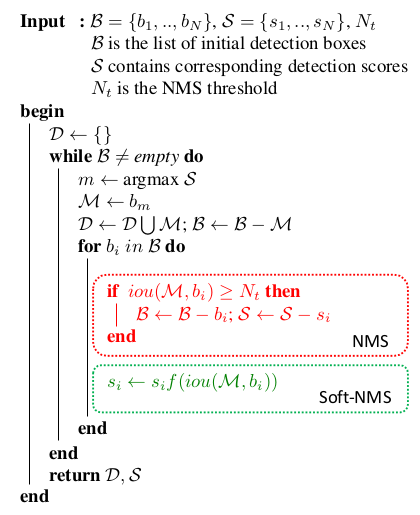
\includegraphics[width=0.5\linewidth]{images/nms_algo.png}
    \caption{Pseud code of NMS and soft-NMS, source \cite{Bodla2017}}
    \label{alg:nms}
\end{figure}

\subsubsection{Soft non-maximal suppression {S-NMS}}
Soft non-maximal supression extends the NMS algorithm by a possibility to keep overlapping the predictions if their confidences are high. Instead of removing boxes with an overlap, we decrease their confidence value by the follwing Gaussian penalty function:
\begin{align}
    s_i = s_i e^{-\frac{\text{iou}\left( \mathcal{M}, b_i \right)^2}{\sigma}}, \forall b_i \notin \mathcal{D}
\end{align}
where $\mathcal{M}$ is the currently processed bounding box, and $\mathcal{D}$ is the set of already processed boxes. After processing all boxes, those with $s_i < T$ are removed, where $T$ stands  for a confidence cut-off threshold \cite{Bodla2017}.

\subsubsection{Non-maximum weighted suppression (NMW)}
Non-maximum weighted suppression does not remove boxes in case of an overlap, but merges them togehter by following formula:
\begin{align}
    \mathcal{M} & = \frac{\sum_{i=1}^n \omega_i \times b_i}{\sum_{i=1}^n \omega_i} \\
    \omega_i    & = s_i \times \text{iou} \left( b_i, b_{ argmax_i s_i} \right)
\end{align}
where $\mathcal{M}$ is the merged bounding box, for which no confidence value is computed \cite{Zhou2017,Solovyev2019}.

\subsubsection{Weighted boxes fusion (WBF)}
Weighted boxes fusion combines boxes similarly to NMW. The main difference is the iterative approach to the fusion, outputting confidence for the merged box, and awareness of several models, which contributed to the prediction.
The steps of WBF are as follows \cite{Solovyev2019}:
\begin{enumerate}
    \item Sort $\mathcal{B}$ by $\mathcal{S}$ as in NMS.
    \item Declare empty lists \boldmath{L} and \boldmath{F} that would be used to store boxes clusters and merged boxes, respectively
    \item Iterate through $\mathcal{B}$. If there is a box in \boldmath{F} for which $IOU > \mathbf{Threshold}$, add the box from $\mathcal{B}$ to list \boldmath{L} on the position corresponding to position of the matched box in \boldmath{F}. If there is no match  found, add it to the end of \boldmath{L}.
    \item Recalculate the box coordinates $\mathcal{M}$ and confidence $c$ in the list \boldmath{F} on the position where we added the box to \boldmath{L} by formulas\ref{eq:wbf1}.
    \item After processing all boxes from $\mathcal{B}$ adjust confidence scores by a formula\ref{eq:wbf2}, where $T$ is the number of contributing boxes and $M$ is the number of models used for ensembling.
\end{enumerate}
\begin{align}
    \mathcal{M} & = \frac{\sum_{i=1}^n c_i \times b_i}{\sum_{i=1}^n c_i} ,\quad c=\frac{\sum_{i=1}^{T}c_i}{T} \label{eq:wbf1} \\
    c           & = c * \frac{T}{M} \label{eq:wbf2}
\end{align}

\chapter{Related Work}
\label{chapter:related_work}
This chapter will introduce relevant publications regarding dental caries detection, focusing mainly on detection from bitewing radiographs. Following that, we will briefly introduce methods for the segmentation of dental restorations.

\section{Dental caries detection}
Since 2017, more than ten publications have been regrading automatic caries detection from images \cite{PradosPrivado2020}. They differ in how they approach caries localization and the types of images they use. The following images have been used: Near-Infrared Transillumination images \cite{Casalegno2019,Schwendicke2020}, camera photographs, \cite{Moutselos2019} and X-ray images, which may be further divided into bitewing \cite{Moran2021, Cantu2020, Bayrakdar2021, Mao2021, Srivastava2017}, panoramic \cite{Lian2021}, and periapical X-ray images \cite{Lee2018}.

All the related publications can be divided into three groups based on their approach to caries localization: Manual detection and classification, dental caries segmentation, and dental caries detection.

\subsection{Manual detection and classification}
This section introduces publications that approached caries detection in the following manner: First, they crop individual teeth from the X-ray image. Manual cropping or non-machine learning computer vision techniques were used for this purpose. After a tooth is extracted from the image, it is labeled by a professional. A classifier is trained on those image patches to decide if it contains a carious lesion.
\begin{itemize}
    \item First attempts to use a neural network for caries detection date back to 2008, when Kuang et al. \cite{Kuang2008} proposed an approach based on passing a patch from an image to a classifier, which then decided if the patch contains caries or healthy enamel. Even though the performance of the proposed neural network was surpassed by 6.72\% by kernel SVM, it was still able to outperform an ordinary dentist by more than 5\%. It was only 6\% worse than an experienced individual.
    \item Moran et al.\cite{Moran2021} used histogram equalization, Otsu's thresholding, and morphological operations to extract individual teeth from bitewing images. After teeth extraction, the dataset was labeled by assigning one of three categories to each tooth. The categories were: Normal teeth, incipient lesions, and advanced lesions. They processed a total of 112 radiographs this way, resulting in 480 teeth with corresponding annotations. Moran et al. trained the ResNet and Inception model to perform the classification task, and the best-achieved accuracy was 73.3\% \cite{Moran2021}.
    \item{Mao at al. \cite{Mao2021}} made a similar preprocessing approach as Moran, only this time extracting unilateral tooth images instead of the whole tooth. A total of 3716 images of unilateral teeth were obtained. AlexNetsed was used for classification and reached a 90.3\% accuracy.
    \item{Lee et al. \cite{Lee2018}} published a similar approach only with periapical images. The dataset with 3000 images was created manually by cropping out teeth from the X-ray image, keeping only those without extensive dental restorations. In the same process, two teeth at once were also cropped from the radiograph. After obtaining this dataset, they trained GoogLeNet and Inception v3 architecture classifiers, obtaining an accuracy of 89\%  for molars and 82\% for images with both premolars and molars.
\end{itemize}


\subsection{Dental caries segmentation}
There are publications where the authors approached the task of caries localization as semantic segmentation. The advantage of this approach is the pixel precision of the lesion detection. On the other hand, creating a similar dataset is very time-consuming. An example of a dataset annotated in a pixel-wise manner is depicted in figure \ref{fig:segmentation_lit} as well as predictions of a model proposed by Cantu \cite{Cantu2020}.

\begin{figure}
    \centering
    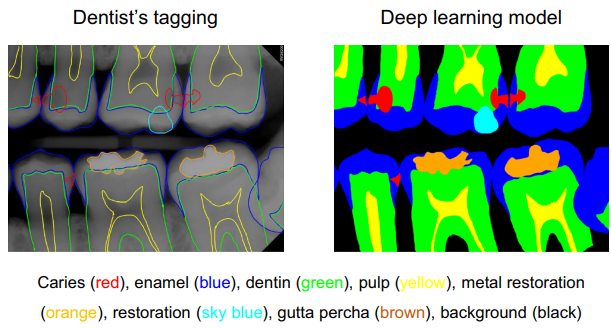
\includegraphics[width=\linewidth]{images/segmentation_bitewing_rich.png}
    \caption{Annotated bitewing radiograph and the same image post-processed, source \cite{Lee2021}}
    \label{fig:bitewing_dense}
\end{figure}

\begin{itemize}
    \item{Cantu et al. \cite{Cantu2020}} created a dataset of 3686 bitewing images. Three dentists drew a polygonal-shaped box over caries independently in each image. In the case of a unanimous decision, the annotation was kept in the dataset. Otherwise, the fourth dentist reviewed the annotation and decided if it should be kept or deleted. Cantu et al. used the U-Net model with EfficientNet B5 as a backbone. They then evaluated the model per pixel, and its performance was compared against seven dentists, outperforming their mean performance in every metric.
    \item{Lian et al. \cite{Lian2021}} had the same approach as Cantu but used panoramic images. In comparison with Cantu, following the segmentation, they cropped the region of interest around the segmented lesion and classified caries into one of four categories as described in the section \ref{sec:caries_classification}. They achieved an IOU score of 0.785 on the segmentation task. In comparison, the best performing dentist achieved an IOU of 0.717. In the classification task, the model outperformed the average dentist's performance.
    \item {Lee at al. \cite{Lee2021}}  approached the problem uniquely. The dataset, consisting of 304 bitewing radiographs, was densely annotated by polygons, denoting the position of dental caries and enamel, dentine, pulp, and gutta-percha restorations. The result of this annotation can be seen in figure \ref{fig:bitewing_dense}. They used two independent U-net models to predict the position of dental caries and remaining structures in the image. The output of both models was post-processed and merged. Even though the model achieved an F1 score of 0.641, which is low compared to other publications, predictions of the model helped dentists improve their sensitivity ratio by 7 - 10\%.
\end{itemize}

\begin{figure}
    \centering
    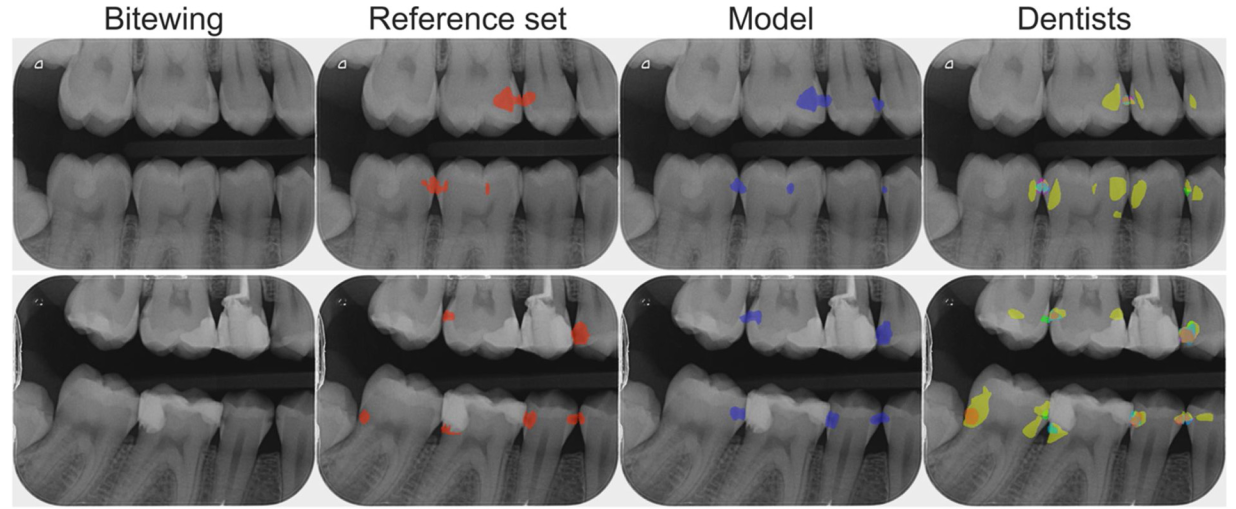
\includegraphics[width=\linewidth]{images/segmentatic_literature.png}
    \caption{Sample of data and predictions of the model by }
    \label{fig:segmentation_lit}
\end{figure}

\subsection{Dental caries detection}
\begin{figure}
    \centering
    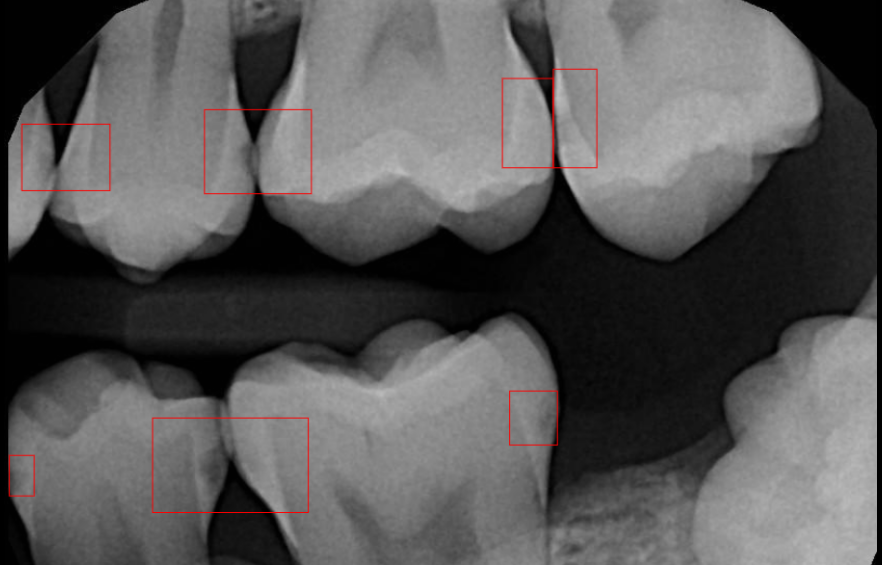
\includegraphics[width=\linewidth]{images/sirvastava_pred.png}
    \caption{Predictions of the model proposed by Srivastava et al., source \cite{Srivastava2017}}
    \label{fig:srivastava_preds}
\end{figure}
\begin{itemize}
    \item{Srivastava et al. \cite{Srivastava2017}} trained a fully convolutional neural network with over 100 layers on a dataset containing more than 3000 bitewing radiographs. They denoted the position of tooth decay in a pixel-wise manner. Even though the model predicts output masks in a semantic segmentation fashion, the output is post-processed by fitting a minimal bounding rectangle around the prediction, as can be seen in figure \ref{fig:srivastava_preds}. After that, the model is evaluated by computing the IOU of the rectangle with the ground truth polygon. If the IOU is greater than 0.8, the detection is considered positive. Srivastava et al. claim that their model outperforms each of the three dentists included in the study considerably. Detailed results are in table \ref{tab:srivastava_results}.

          \begin{table}
              \centering
              \begin{tabular}{c||c|c|c|c|c}
                  Metric    & Model \cite{Srivastava2017} & Model \cite{Kumar2018} & Dr. 1 & Dr. 2 & Dr. 3 \\ \hline
                  Recall    & 0.805                       & 0.70                   & 0.477 & 0.433 & 0.344 \\ \hline
                  Precision & 0.615                       & 0.53                   & 0.63  & 0.815 & 0.891 \\ \hline
                  F1-Score  & 0.70                        & 0.614                  & 0.54  & 0.56  & 0.50
              \end{tabular}
              \caption{Results of models proposed in \cite{Srivastava2017} and \cite{Kumar2018}, compared with three dentists, modified}
              \label{tab:srivastava_results}
          \end{table}

    \item{The same author and Kumar \cite{Kumar2018}} published another paper, where they changed the model to U-Net, which was trained on an extended dataset of 6000 bitewing X-ray images. The authors tested the hard example mining approach, but it led to a decrease in performance. Even though U-Net architecture usually achieves better results on publicly available benchmarks \cite{paperwithcode, Zhang2019}, and the size of the dataset increased twofold, the model's performance dropped by 15\%, see table \ref{tab:srivastava_results}. There is no information available about the evaluation protocol used by Kumar \cite{Kumar2018}, nor about the IOU threshold needed to consider a prediction to be correct. This makes it hard to estimate the cause of the performance drop.
    \item{Barakdar et al. \cite{Bayrakdar2021}} did both semantic segmentation and object detection. A dataset of 621 bitewing images was available for both of those tasks. They claim to use U-net for segmentation and VGGNet for object detection. The paper does not mention how they modified the VGGNet architecture for object classification to perform an object detection task. The object detection results were evaluated against five professionals in dentistry with different years of experience. The model has outperformed two dentists with two and three years of experience while being outperformed significantly by all three dentists with ten years of experience. The reported precision of the model is $0.78$, recall=$0.77$ and F1 score of $0.78$. The paper has no information about the overlap used to consider predictions to be correct. We assume it was set to be $0.5$.
    \item{Bayraktar2021 er al. \cite{Bayraktar2021}} solved only the object detection task on a dataset of 1000 bitewing images labeled by two experts with more than ten years of experience. With YOLOv3 architecture model, they achieved $AP@.5 = 0.872$ .
\end{itemize}

\section{Dental restorations segmentation}
\label{sec:related_works:dental_restorations}
To the author's knowledge, no available publications are regrading the segmentation of dental restorations in bitewing radiographs. Therefore, we will introduce two methods that segment dental caries from panoramic X-ray images. Figures \ref{fig:restoration_seg_pub1}, \ref{fig:restoration_seg_} contain samples of images used for restoration segmentation.
In addition, we will mention two publications where restoration detection was a minor part of the work.
\begin{figure}
    \begin{floatrow}[2]
        \ffigbox[1.25\FBwidth]{\caption{Results of segmentation algorithm proposed by Yeshua et al.\cite{Yeshua2019}}\label{fig:restoration_seg_pub1}}%
        {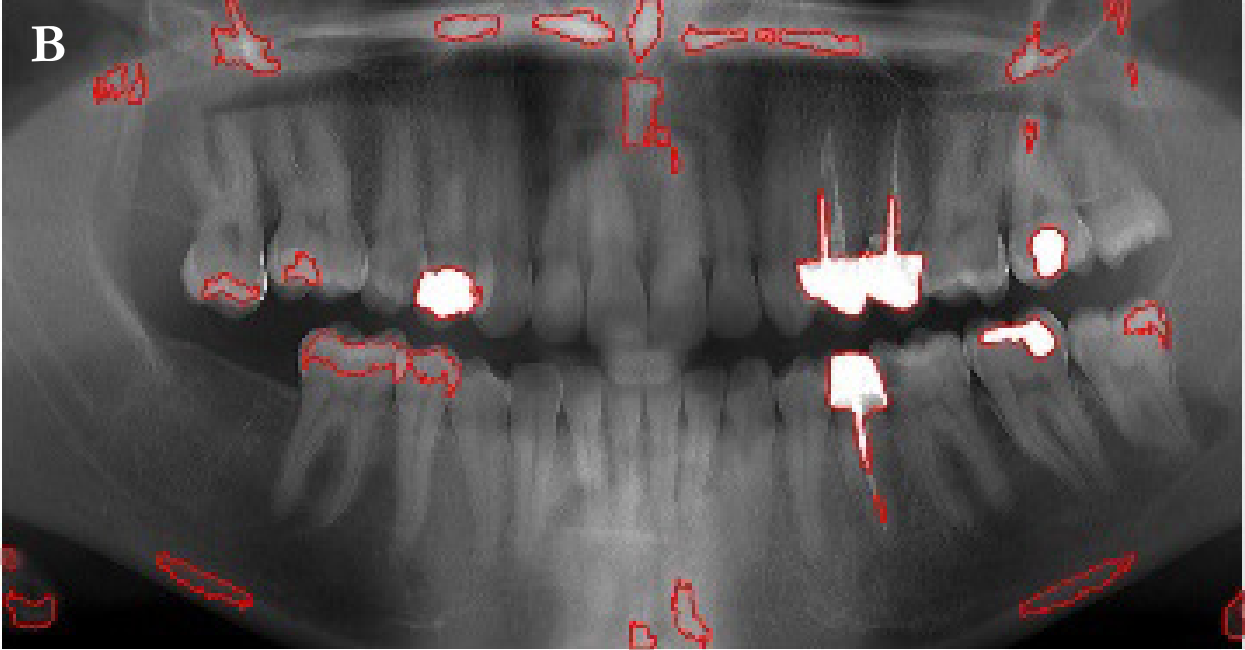
\includegraphics[width=\linewidth]{images/segmentation_opg.png}}\;
        \ffigbox[0.75\FBwidth]{\caption{Cropped region from panoramatic image with multiple restorations, source \cite{AbdallaAslan2020}}\label{fig:restoration_seg_pub2}}%
        {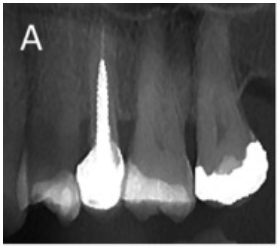
\includegraphics[width=\linewidth]{images/segmentation_crop.png}}
    \end{floatrow}
\end{figure}
\begin{itemize}
    \item{Mao et al. \cite{Mao2021}} classified dental segmentations in previously extracted image patches with unilateral teeth.
    \item{Lee at al. \cite{Lee2021}} did not focus directly on the segmentation of restorations, but it was one of the classes segmented out by their U-net architecture. There are no metrics available regarding the algorithm's performance on dental restorations.
    \item{Abdalla-Aslan et al. \cite{AbdallaAslan2020}} used methods of classical computer vision to segment out restorations in panoramic images. Their pipeline consisted of: Adaptive gaussian thresholding, morphological operations, and deleting regions in peripheral areas of the image. The final algorithm had the precision and sensitivity of 0.33 and 0.946, respectively. After successful detection, the restoration was classified as: dental implant, crown, amalgam filing, etc.
    \item {Yeshua et al. \cite{Yeshua2019}} solved the same problem as Abdalla-Aslan. Even the approach was more-less the same, but their solution achieved a precision of 0.568. They classified detected areas similarly to Abdalla-Aslan, having an extra category for false detections. After the removal of false detections, the precision was boosted to 0.98.
\end{itemize}
\chapter{Dataset}
\label{chapter:dataset}
Altogether,  MDDr. Tichý and his team created two datasets. One dataset was used to detect dental caries and the other for semantic segmentation of dental restorations. The majority of work was done on the first-mentioned set of data.

\begin{figure}
    \centering
    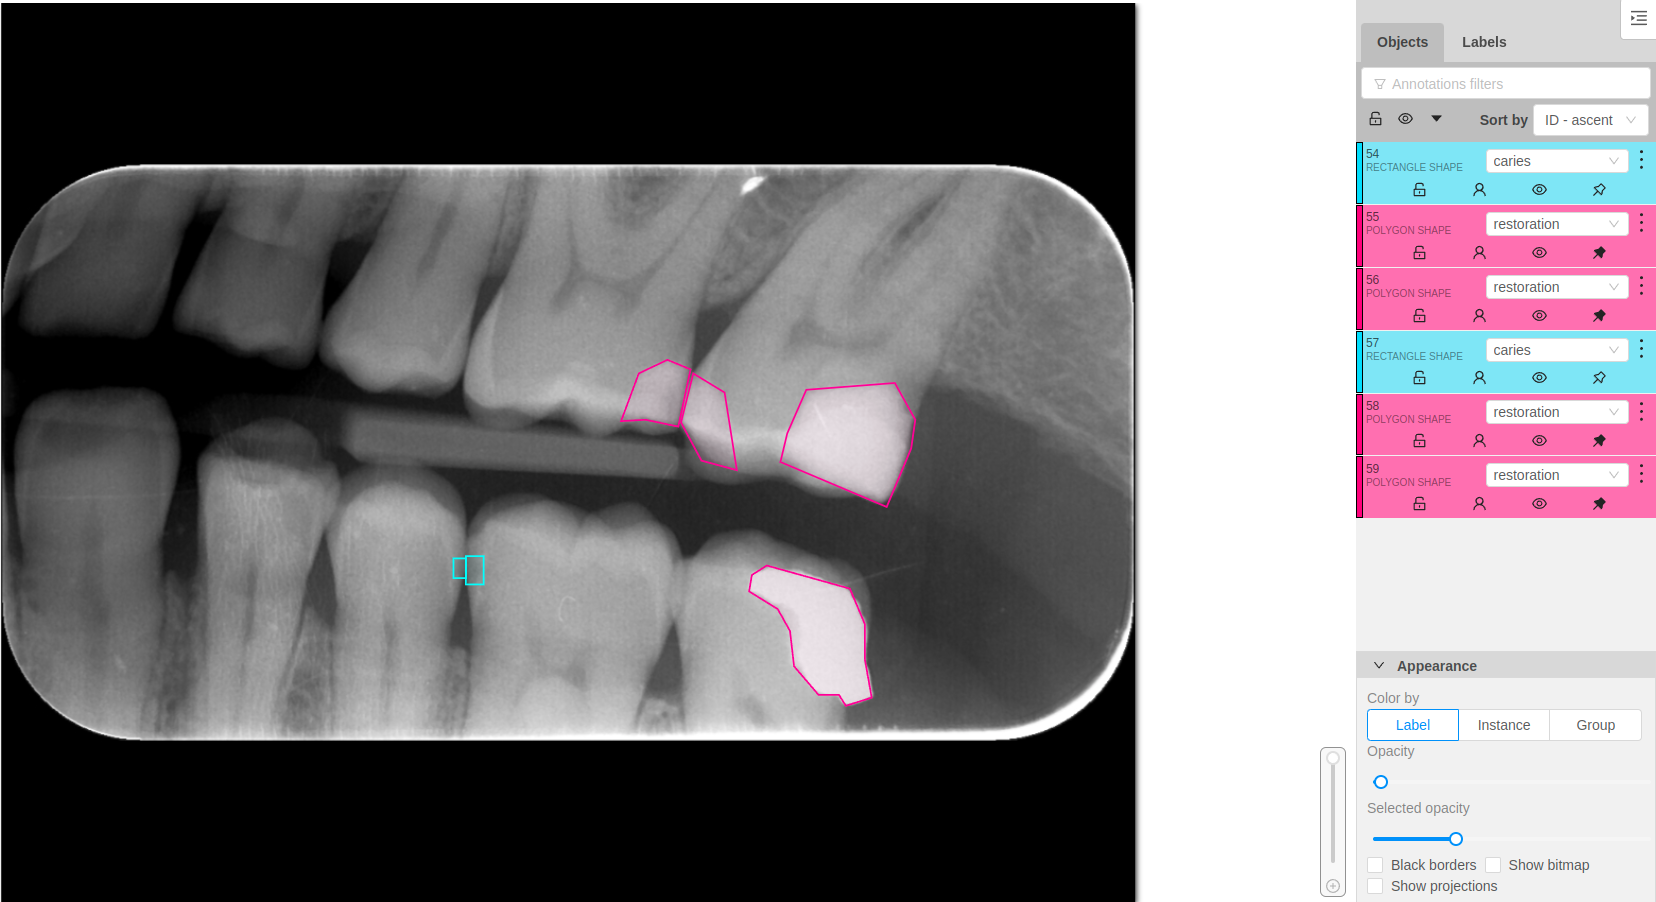
\includegraphics[width=\linewidth]{images/cvat.png}
    \caption{The environment of CVAT with annotated carious lesion and dental restorations}
    \label{fig:cvat}
\end{figure}

\section{Dental caries}
MDDr. Tichý and his team began to work on the datasets in September of 2021, along with the beginning of work on this thesis. This led to an opportunity to discuss the format of the data. We decided to annotate every dental caries lesion with a minimal bounding box. The annotation process was conducted in the Computer Vision Annotation Tool (CVAT), running on the Faculty of biomedical informatics server. The web address is www.gdiag.fbmi.cvut.cz.

While denoting the position of the carious lesion, the annotator tried to be consistent with the following guidelines:

\begin{itemize}
    \item Carious lesion is marked by a rectangle. The rectangle should contain the entire lesion while remaining as small as possible at the same time.
    \item When the lesion is on the proximal surface, and both teeth are infected, draw a separate box for each of them.
\end{itemize}

Due to constant work on the dataset, we decided to use the same data as long as there was no major update leading to a release of an improved dataset. We call these releases the stages of the dataset. In total, six major releases were done. This ensured that we were able to compare the performance of our models to each other on different stages of the dataset. 

\subsubsection{First stage}
In the very first stage MDDr. Tichý instructed a group of general dentistry students on how to approach the annotation to get as homogenous dataset as possible. They then annotated a couple of images under his supervision before continuing independently.
Dental X-ray images were uploaded into CVAT and divided into multiple projects, where each project contained between 400-800 images. This was essential due to technical limitations regarding exporting and uploading X-ray images from a dental database. We further split each project into jobs consisting of 100 images each and assigned them to a particular student. We had 1695 X-ray images at our disposal with 2416 dental caries annotated when the first stage was done.
CVAT does not allow exporting and merging multiple tasks, so we exported each task separately in COCO format. We uploaded all images and files with annotations  to the CMP server. The server contains annotations combined in one annotation.json file, which carries the information about the dataset in COCO format, and one folder with all the images. We checked the task for duplicates and non-reviewed radiographs and removed those, which resulted in 1626 images with 2399 decay annotations. Out of those, 946 images contained at least one cavity.


\subsubsection{Second stage}
After inspection of the dataset created in the first stage, we observed in-homogeneity across the annotations. Some of the guidelines were violated, especially the one regarding caries on proximal surfaces. In addition, we observed multiple overlooked lesions. This led us to a reconsideration of our approach to labeling and MDDr. Tichý himself did all the annotation work from this moment further on. After the second stage, the dataset was extended to 2599 non-duplicate images containing 4328 annotations of tooth decay. In this stage, we did no corrections of previous errors.

\subsubsection{Third stage}
MDDr. Tichý reviewed all images annotated in the first stage, removing as well as adding an unspecified amount of annotations. In the end, the dataset consisted of 2599 images with 4575 annotations of dental caries.

\subsubsection{Fourth stage}
We uploaded another 1400 images onto the CVAT server. All the images were downloaded and uploaded to the CMP server. We used a  YOLOv5 model\footnote{For further information about the performance of the model, see table \ref{tab:model_results:stage_three:test}} trained on the third stage dataset to generate predictions for each image. Confidence threshold maximizing F1 score on the validation dataset was used to filter out low confidence predictions of the model. We used Voxel Fiftyone tool to upload all 1400 images and their respective predictions to CVAT, where those images were split into two separate tasks.
MDDr. Tichý reviewed all predictions and conducted adjustments of bounding boxes as well as their removal and addition.  According to his personal statistics, there were roughly 200 predictions per 100 images. Around 20 predictions had to be added and removed to get the same quality annotations as in stage three. The upside of using model prediction as a starting point for the annotation process was the speed. The annotation was done in approximately half the time required to do the annotation without model predictions. In total, 3500 images were available after this stage. After removing corrupted images, we got 3489 X-rays with 6087 annotations.

\begin{figure}
    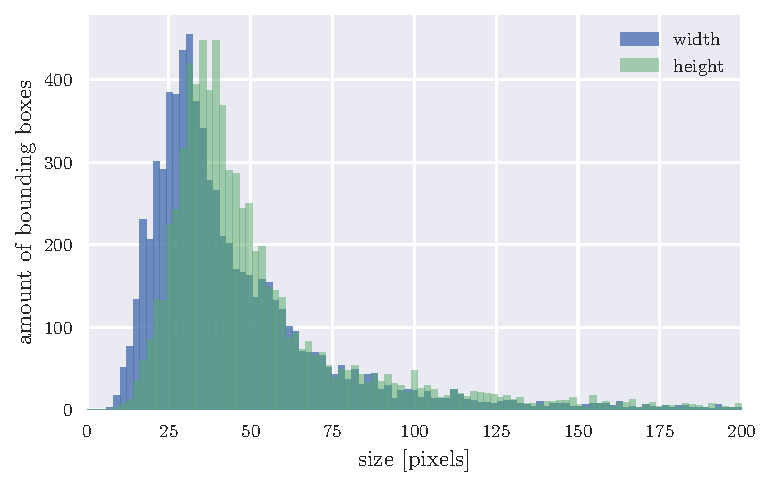
\includegraphics[width = 0.9\linewidth]{images/dataset_histogram.pdf}
    \caption{Histogram of bonding boxes dimensions in the dataset}
    \label{fig:hist_caries_dim}
\end{figure}

\begin{figure}
    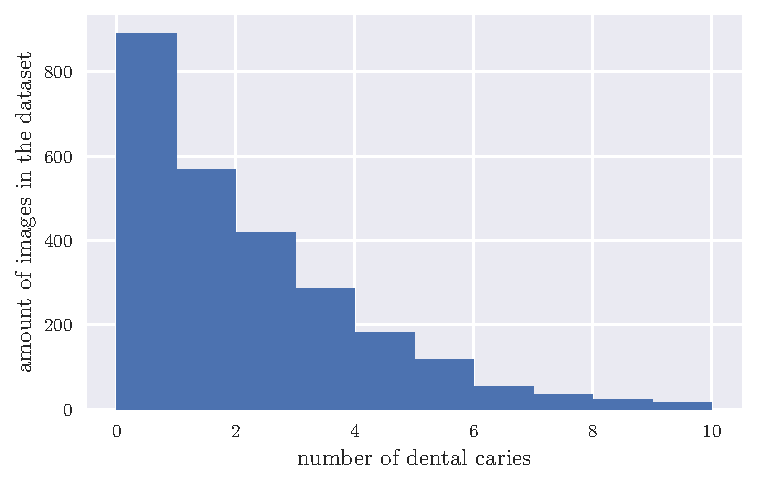
\includegraphics[width=0.9\linewidth]{images/caries_histogram.pdf}
    \caption{Histogram of the number of dental caries per image}
    \label{fig:hist_caries_per_img}
\end{figure}
\subsubsection{Image augmentations}

\subsubsection{Fifth stage}
In this stage, we finished the annotation of all 1400 images uploaded in stage four, resulting in 3989 X-rays with 7257 annotations. We plotted a histogram representing the distribution of the number of carries among images; it can be noticed in figure \ref{fig:hist_caries_per_img}.


\begin{table}
    \centering
    \begin{tabular}{|l|r|r|}
        \hline
                                       & Width [px] & Height [px] \\\hline
        Image size                     & 1068       & 795-847     \\ \hline
        Minimal box size               & 8          & 9           \\ \hline
        Maximal box size               & 384        & 315         \\ \hline
        Mean of box size               & 47.55      & 53.15       \\ \hline
        Standard deviation of box size & 37.99      & 35.33       \\ \hline
    \end{tabular}
    \caption{\label{tab:dataset_statistics}Statistics of bounding boxes, that denote position of carious lesions}
\end{table}

\subsubsection{Sixth stage}
We evaluated the model's performance on the test, validation, and training part of the dataset. Although the model used for prediction achieved $AP@.5 = 0.72$, there were 1598 images with at least one false positive or false negative detection. We decided that doing a second round of dataset review would be more beneficial than further expansion of the size of the dataset. We focused only on erroneous images and uploaded those 1598 images with no  less than a single error to the CVAT annotation tool for review. When writing this thesis, there is still undergoing work on the uploaded images. Therefore, we were not able to use the sixth stage.


\section{Dental restorations}
\begin{figure}
    \centering
    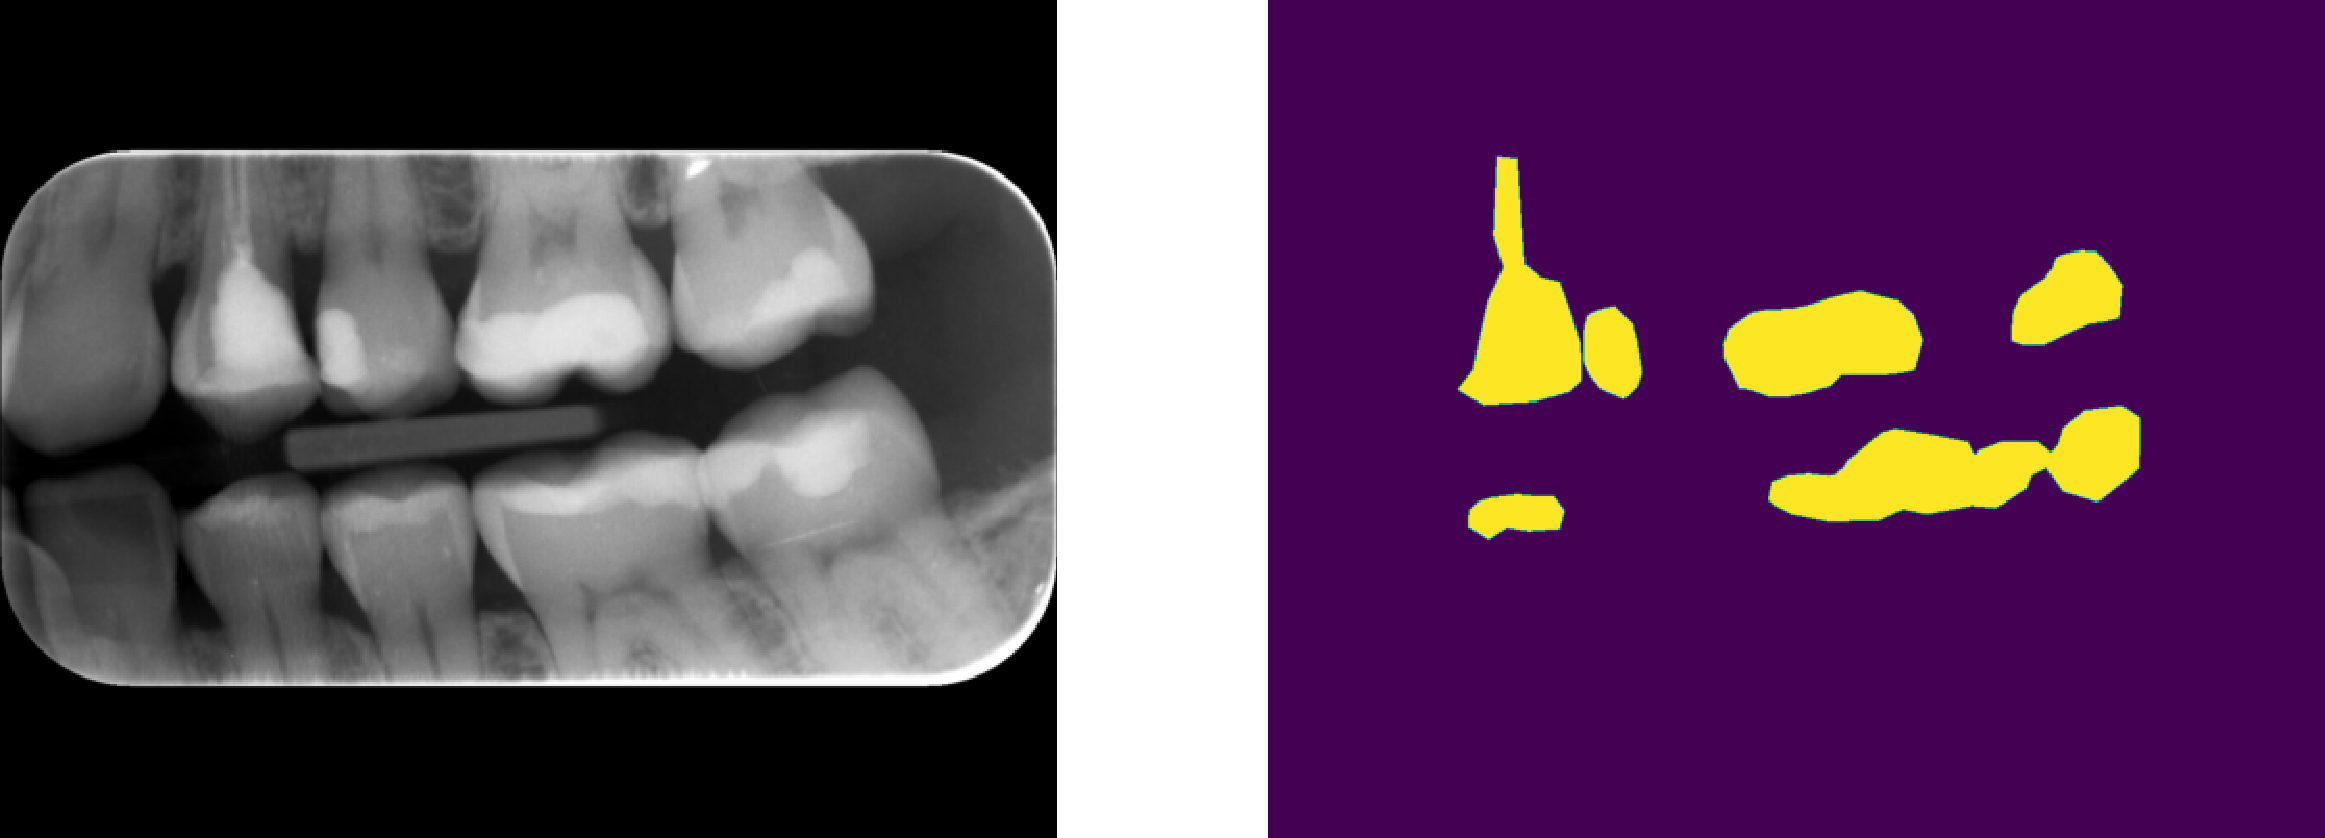
\includegraphics[width=\linewidth]{images/segmentation_ds_sample.pdf}
    \caption{Bitewing X-ray image on the left, pixel mask of the X-ray on the right (dental restorations have yellow color)}
    \label{fig:segmentation_sample}
\end{figure}
This dataset consists of a subset of images used in the dental caries dataset. MDDr. Tichy's  team annotated it in the CVAT tool by drawing a polygon around each dental restoration. The work was done by the same group of dentistry students as stage one of the caries dataset and reviewed by a single fifth-year dentistry student. Evaluation of the whole dataset performed by a single person should ensure consistency among images. A total of 521 images were used to create this dataset, and an inspection revealed that 387 radiographs contained at least a single annotated restoration, and 134 had none.
The dataset was exported from CVAT in COCO format and saved on the CMP server. When working with the data, we used a pixel mask instead of polygons to denote the position of dental restorations. A sample of the dataset with a pixel mask is  featured in figure \ref{fig:segmentation_sample}.

In figure \ref{fig:segmentation_restoration_size} we can  notice how many percent of the X-ray image consists of restorations. This gives us an idea of how common dental restorations in our data are. In figure \ref{fig:segmentation_patch_size} we see how the size of each restoration is distributed. Inspecting this figure, we observe that most restorations are smaller than $2\%$ of the image.

\begin{figure}
    \centering
    \begin{floatrow}[2]
        \ffigbox[\FBwidth]{\caption{Histogram of restoration area in image, images without restorations omited}\label{fig:segmentation_restoration_size}}%
        {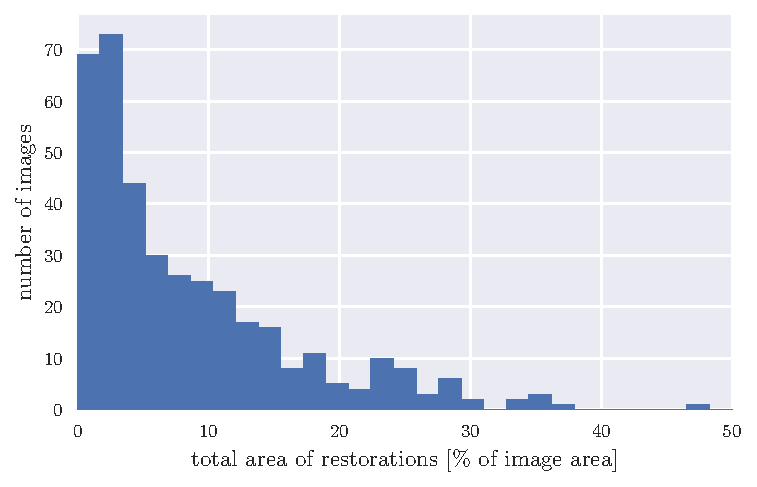
\includegraphics[width=\linewidth]{images/histogram_of_restoration_size.pdf}}\;
        \ffigbox[\FBwidth]{\caption{Histogram of areas of restorations, 10 largest omited}\label{fig:segmentation_patch_size}}
        {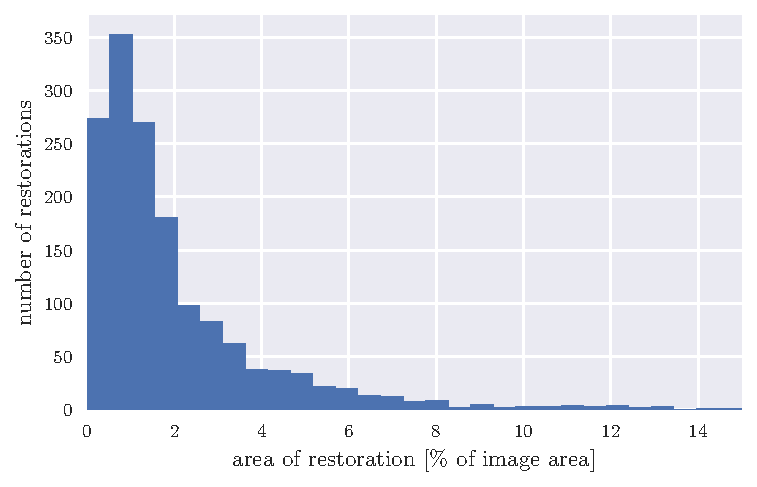
\includegraphics[width=\linewidth]{images/histogram_of_patch_size.pdf}}
    \end{floatrow}
\end{figure}
\chapter{Project structure}
\label{chapter:project_structure}

\section{Organization of the project}

\begin{figure}
    \centering
    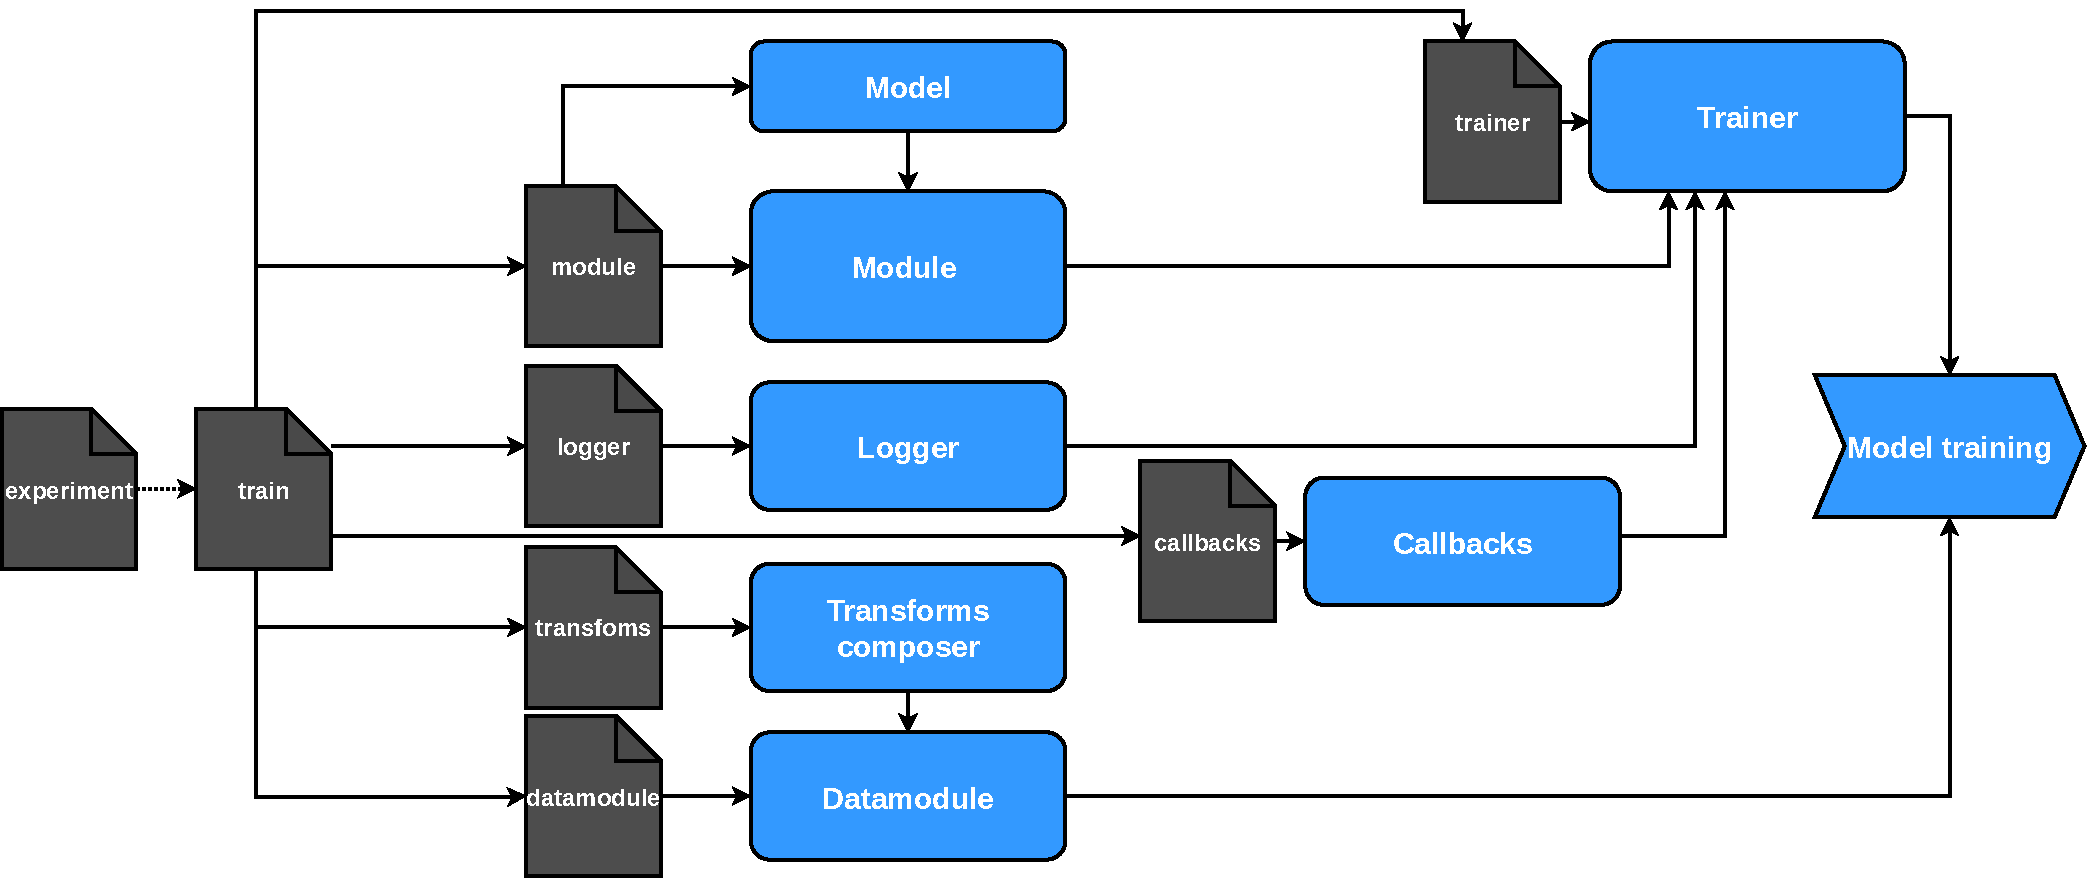
\includegraphics[width=\linewidth]{images/Module.drawio.pdf}
    \caption{Structure of modules and their configuration files}
    \label{fig:structure_modules}
\end{figure}

\begin{figure}
    \begin{forest}
        for tree={
        font=\ttfamily,
        grow'=0,
        child anchor=west,
        parent anchor=south,
        anchor=west,
        calign=first,
        inner xsep=7pt,
        edge path={
                \noexpand\path [draw, \forestoption{edge}]
                (!u.south west) +(7.5pt,0) |- (.child anchor) pic {folder} \forestoption{edge label};
            },
        before typesetting nodes={
                if n=1
                    {insert before={[,phantom]}}
                    {}
            },
        fit=band,
        before computing xy={l=15pt},
        }
        [MT
            [configs - root folder with all configuration files
                    [callbacks]
                    [datamodule]
                    [experiment]
                    [logger]
                    [module]
                    [trainer]
                    [transforms]
                    [train.yaml]
            ]
            [src - folder with all source files
                    [core - structures for data manipulation]
                    [data - utility functions for dataloaders and datasets]
                    [datamodules]
                    [models]
                    [modules]
                    [notebooks - \text{jupyter notebooks for auxilary tasks}]
                    [transforms - \text{classes to compose transformations given by configuration file}]
                    [utils  - \text{functions for logging, losses, data conversion}]
            ]
            [tests - contains multiple subfolders with unit tests for the program]
        ]
    \end{forest}
    \caption{Folder structure of the project}
    \label{fig:folder_structure}
\end{figure}
We wrote the object detection framework developed for this project in Python 3.8.12 programming language \cite{Python}. We structured it into multiple independent modules, which can be swapped for their  corresponding alternatives. This ensures maximal reuse of the written code and allows further extension of this framework. This modular approach was inspired by MetaAI research \cite{MetaAIStatement} and IceVision library \cite{Icevision2022}. The framework's modularity will enable us to use it for semantic segmentation or classification problems.
The core of the project is the deep-learning framework PyTorch 1.11.0 \cite{Pytorch}, which is used to create and train neural networks. Although there are many open-source libraries with object detection frameworks, it is far from optimal to rely only on those libraries since the options to change the program's behavior are limited.
We, therefore, decided to write our own. The framework handles all tasks required for training a model: Loading the data, model definition, optimization of the model, tracking the progress of training, etc.  Implementing all models from scratch would be a waste of time; therefore, we support third-party models' usage. However, only the bare model is used. Thus, we can change everything except for the architecture of the model and its forward pass.

The project is divided into three folders: configurations, tests, and source (src). The first mentioned contains YAML files that are further dispersed into dedicated folders based on the module they configure. At the root of the configurations folder are train.yaml and test.yaml files, which define how to compose individual modules to perform the target tasks. Hydra \cite{Yadan2019Hydra} handles the composition of configuration files. The user can override the default configuration from the command line or experiment.yaml file. The whole configuration pipeline can be seen in figure \ref{fig:structure_modules} and the project's folder structure is in figure \ref{fig:folder_structure}.



\subsection{Models}
Models are implementations of one of the architectures described in section \ref{sec:deteciton_models}. We can either fully implement them, or we can rely on open-source libraries. In that case, we need to implement a function that transforms the data into the format required by the third-party model.

\subsection{Modules}
Modules are a wrapper around the model based on Pytroch-Lightning modules \cite{falcon2019pytorch}. In modules, we take care of the following:
\begin{itemize}
    \item Training and validation loop
    \item Initialization of optimizer
    \item Initialization of learning rate schedulers
    \item Computing metrics
    \item Logging metrics to a predefined logger
    \item Transformations of outputs of models into the unified format
\end{itemize}


\subsection{Transformations}
Transformations are defined by their YAML configuration file. This file is passed to the transforms composer class, which creates training and validation transformations passed to a data module. We relied on the Albumentations library for the individual augmentations.

\subsection{Data-Modules}
Data modules are based on PyTorch-Lightning data modules. It consists of:
\begin{itemize}
    \item Dataset, where we load the data from the hard drive into the memory and pars the file with saved annotations. After loading the data, predefined transformations are applied.
    \item Functions that transform the loaded data into the format required by the model we are about to train.
    \item Definitions of data loaders, which are responsible for merging the data into chunks, so-called batches.
\end{itemize}
\subsection{Trainer}
Trainer defines properties of the training such as the number of GPUS used for the training or a maximal number of epochs that training is allowed to take before terminating.

\subsection{Callbacks}
Callbacks add capabilities to the training pipeline without changing any code. Typical ones that we used were: Definition of stopping criteria, adjusting policy for saving weights of the model, or saving images with their predictions during the training.

\subsection{Logging}
A logger is software capable of storing and visualizing logged values. In the beginning, we used Tensorboard TODO, but soon we switched to Weights and Biases \cite{wandb} and used them throughout the rest of the thesis.

\section{Additional open-source software}
Throughout the project, we used the libraries mentioned above as well as the following:
\begin{itemize}
    \item OpenCV \cite{opencv_library}  computer vision library during the segmentation of dental restorations for operations such as: Adaptive thresholding, morphological operations, etc.
    \item Computer vision library Kornia \cite{eriba2019kornia} was used to perform morphological operations on PyTorch tensors quickly.
    \item MMDetection \cite{mmdetection} provides an implementation of multiple object detection models. We used their implementation of swin transformers, RetinaNet and Faster-RCNN
    \item During the computation of metrics, we used PyCOCOtools, an official \cite{pycocotools} implementation of MS COCO metrics, which had to be significantly modified to provide us with the required capabilities.
    \item To visualize predictions, we used Voxel Fiftyone \cite{moorefiftyone}. The program can be on a self-hosted server. We used this to share predictions of the model with MDDr. Tichý, who was thus able to assess those and decide if the dataset contains any erroneous annotations
    \item For model ensembling, we used the methods implemented by the author of Weighted box fusion \cite{Solovyev2019}. We further enhanced the capabilities of their methods.
    \item We used YOLOv5 models from the Ultralytics repository \cite{glennjocher2020}.
\end{itemize}
% \chapter{Methods}
\section{Dataset}
The dataset was created by Dr. Tichy and his team using the Computer Vision Annotation Tool (CVAT). It has been extended and improved multiple times over the course of this work, and there is still ongoing work. At the time of writing this report, it consisted of 2599 bitewing X-ray images with 4575 annotations of tooth decay. Out of those, there are 890 images without any decay. The distribution of dental caries per image is depicted in the figure \ref{fig:hist_caries_per_img}. For clarity reasons, we omitted 6 images that contained more than 10 caries. From the histogram on the figure \ref{fig:hist_caries_dim}, we observe that most of the caries have dimensions between 10 and 75 pixels. However, there are outliers as big as 380 pixels per dimension. This diversity is increasing the difficulty of the task.

We used the COCO data-format to store data, and used the format during the whole work only with rare exceptions when custom data-format was needed. During the experiments, we used the 70:15:15 split into training, validation and test dataset.
\begin{figure}
    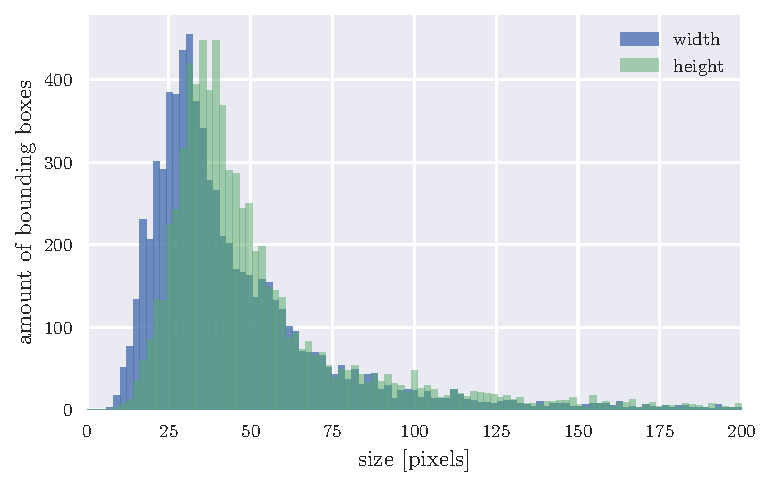
\includegraphics[width = \linewidth]{images/dataset_histogram.pdf}
    \caption{Histogram of bonding boxes dimensions in the dataset}
    \label{fig:hist_caries_dim}
\end{figure}

\begin{figure}
    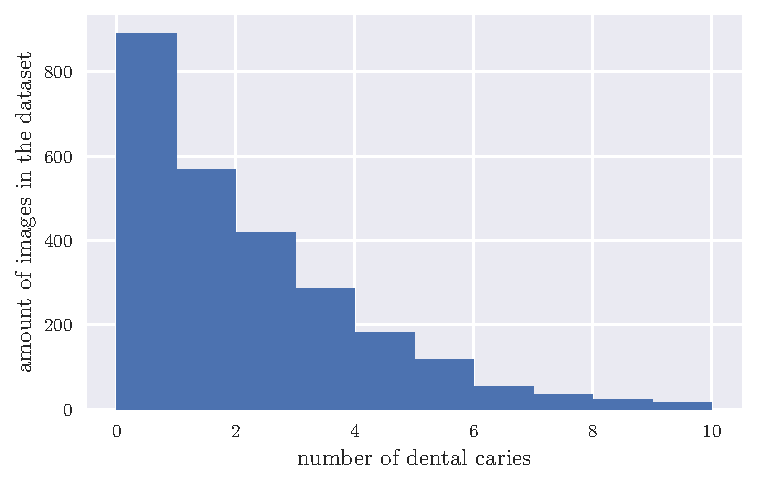
\includegraphics[width=\linewidth]{images/caries_histogram.pdf}
    \caption{Histogram of the amount of dental caries per image}
    \label{fig:hist_caries_per_img}
\end{figure}

\section{Neural network models}
% \chapter{Results}

\section{Different backbones}
We changed the batch-size to 2 (to be able to fit 5x6 backbone into the GPU memory) and trained the model with different bacbones for 50 epochs each. Results for all runs are in the table \ref{tab:yolov5_backbones}.

\begin{table}
    \begin{tabular}{c|c|c|c|c|c}
        Backbone & $AP@.5$ & $AP$  & Parameters[M] & Flops[G] & Time[h] \\ \hline
        5s6      & 0.593   & 0.231 & 12            & 21       & 2.1     \\ \hline
        5m6      & 0.621   & 0.242 & 35            & 63       & 3.5     \\ \hline
        5l6      & 0.611   & 0.241 & 76            & 141      & 5.2     \\ \hline
        5x6      & 0.601   & 0.238 & 140           & 267      & 8.5     \\
    \end{tabular}
    \caption{Results of the YOLOv5 architecture with different backbones}
    \label{tab:yolov5_backbones}
\end{table}

\section{Different image size}
Once again we kept the same setting and this time changed only the size to which images are resized. The relation between input image size and $AP@.5$ can be observed in the figure

\begin{figure}
    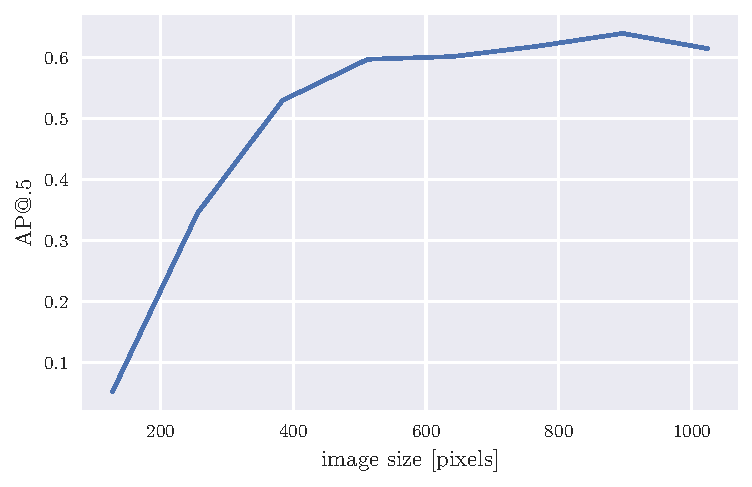
\includegraphics[width=\linewidth]{images/img_size_dependency.pdf}
    \caption{Dependency of $AP@.5$ on the input image size}
\end{figure}

\chapter{Discusion and further suggestions}
\section{Discusion}
From the results in chapter \ref{chapter:results} and figures in appendix \ref{appendix:model_predictions}, we can see that the model is able to localize large portions of dental caries in the image, yet there is still a room for improvement.

\begin{itemize}
    \item In figure \ref{fig:yolov5_map_iou_thresholds}, we can see a sharp drop in the MAP values when IOU threshold greater than 0.4 is chosen. It is observable in both training and validation MAP. This seems to be related to the data rather than to the model. Also, it matches the expectations of Dr.Tichy, who said that in many cases it is not crystal clear where exactly the tooth decay is located, and there is thus slight ambiguity in the image labeling.
    \item From predictions in figures \ref{fig:pred_img1}, \ref{fig:pred_img2}, \ref{fig:pred_img3}, \ref{fig:pred_img4}, we can see that the model is incapable of precise predictions in the vicinity of dental restorations. This is a common pattern accros the whole dataset and is probably caused by a high variety of restorations shapes as well as by the low amount of similar images in the dataset.
    \item The best performing YOLOv5 backbone was not the biggest one, but the 5m6 backbone, which is considered to be a medium sized option. Even though the difference was negligible, it is still an unexpected result, that the 5m6 backbone was albe to outperform 5x6 backbone, even though it achieved by 10 \% better results than 5m6 when benchmarked on the MS COCO dataset \cite{glennjocher2020}. The inability to utilize the bigger backbone can be caused by a wrong setup of the training pipeline or the low amount of data.
    \item There was a drop of the model performance when selecting the image size of 1024 over 896. Even though the difference is subtle, we would expect the opposite.
    \item Even though in MS COCO benchmark EfficientDet-D4, there is a better performing model than in YOLOv5-5l6, it has shown to be worse performing on our dataset. This could be caused by extremely low batch size of 1.
\end{itemize}
\section{Suggestions for further work}
Right now, there seems to be no straightforward way to improve the performance significantly. We could try to do the hyper-parameter search, but personally I would resort to this option later.

We could try different architectures since the best performing YOLOv5 is not state-of-the-art \cite{paperwithcode}. YOLOR and the newest versions of YOLOv4 are outperforming YOLOv5 by 12\% and 10\%.

We could modify the training pipeline by, for instance, changing the optimizer and the learning rate scheduler.

We could try to do image preprocessing or try automatic augmentation search as proposed by Cubut et al. \cite{Cubuk2018}.

Methods that almost always improve the performance are model ensembling and test-time augmentations. We could try how big performance bump they would provide in our problem.
\chapter{Conclusion}

This thesis has developed a solution based on convolutional neural networks for the purpose of dental caries detection and dental restorations segmentation. The best-performing model for dental caries detection achieved $AP@.5=0.725$, and an ensemble of ten models improved the results to $AP@.5=0.774$. The best model for dental restorations segmentation achieved an IOU of 0.676 and a Dice score of 0.76.

\medskip
We contributed to the creation of a dataset containing 3989 bitewing images with 7257 annotated dental caries. Furthermore, for 521 images, a pixel mask with highlighted dental restorations is available. To our knowledge, this is one of the most extensive datasets created for caries detection.

\medskip
During the dataset's creation, the model already proved to detect dental caries overlooked by a dentist. Since then, the model has improved significantly. We, therefore, believe that the model in its current state would be helpful during teeth diagnosis. It could serve as a second opinion for the dentists that he can compare his beliefs against.

\section*{Further work}
The primary focus should be on finishing the stage six dataset in the future. We believe that there are still overlooked dental caries in the dataset, despite their number decreasing in stage three.
\medskip
We believe that including an additional model with different architecture could further increase the performance. For example, parameter-heavy models such as EfficientDet could be trained and added to the ensemble. However, this would require a GPU with at least 24GB of dedicated memory.

\medskip
It could be worth exploring the option of backbone sharing across multiple tasks. The model for segmentation of dental restorations could benefit from the backbone shared with the model for object detection, which was trained on a significantly larger amount of data. Therefore, we believe that the backbone would be able to extract better features from the image.







\appendix
\bibliographystyle{IEEEtran}
\bibliography{svp}
\chapter{Images}
\label{apendix:img_transformations}
\begin{figure}
    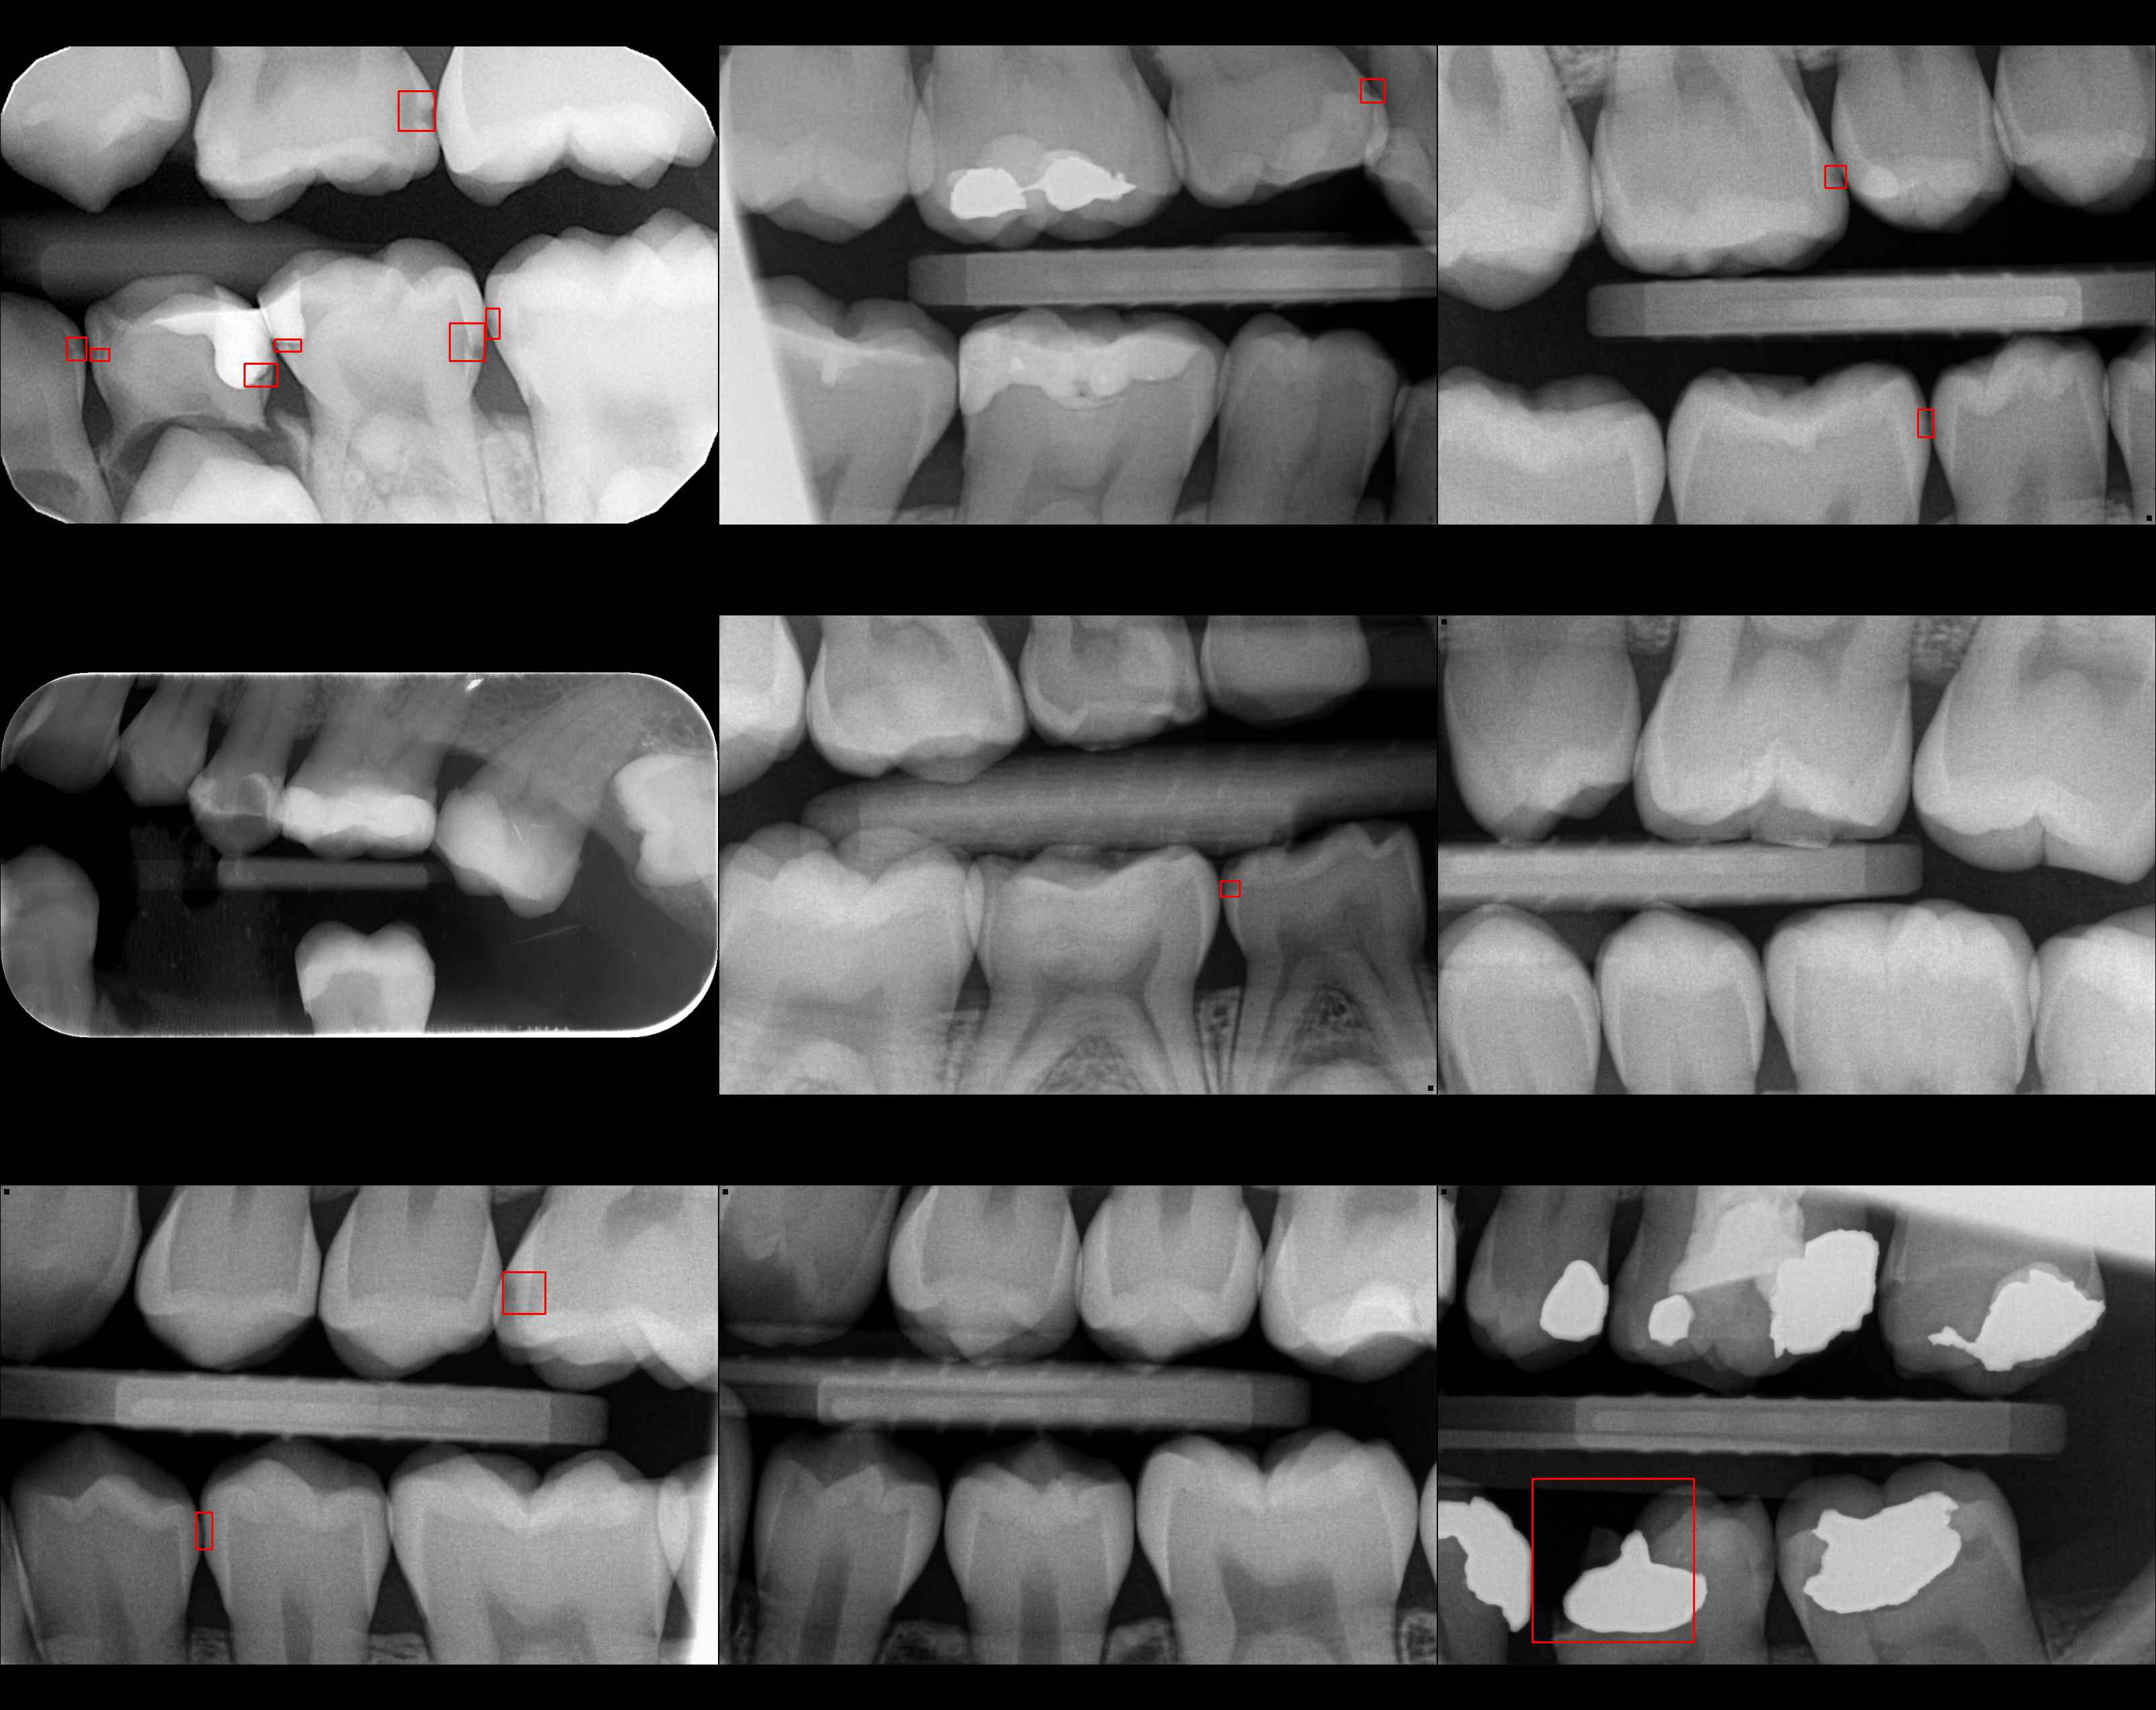
\includegraphics[width =0.9\linewidth]{images/no_trasnforms.jpg}
    \caption{No transformation applied}
\end{figure}
\begin{figure}
    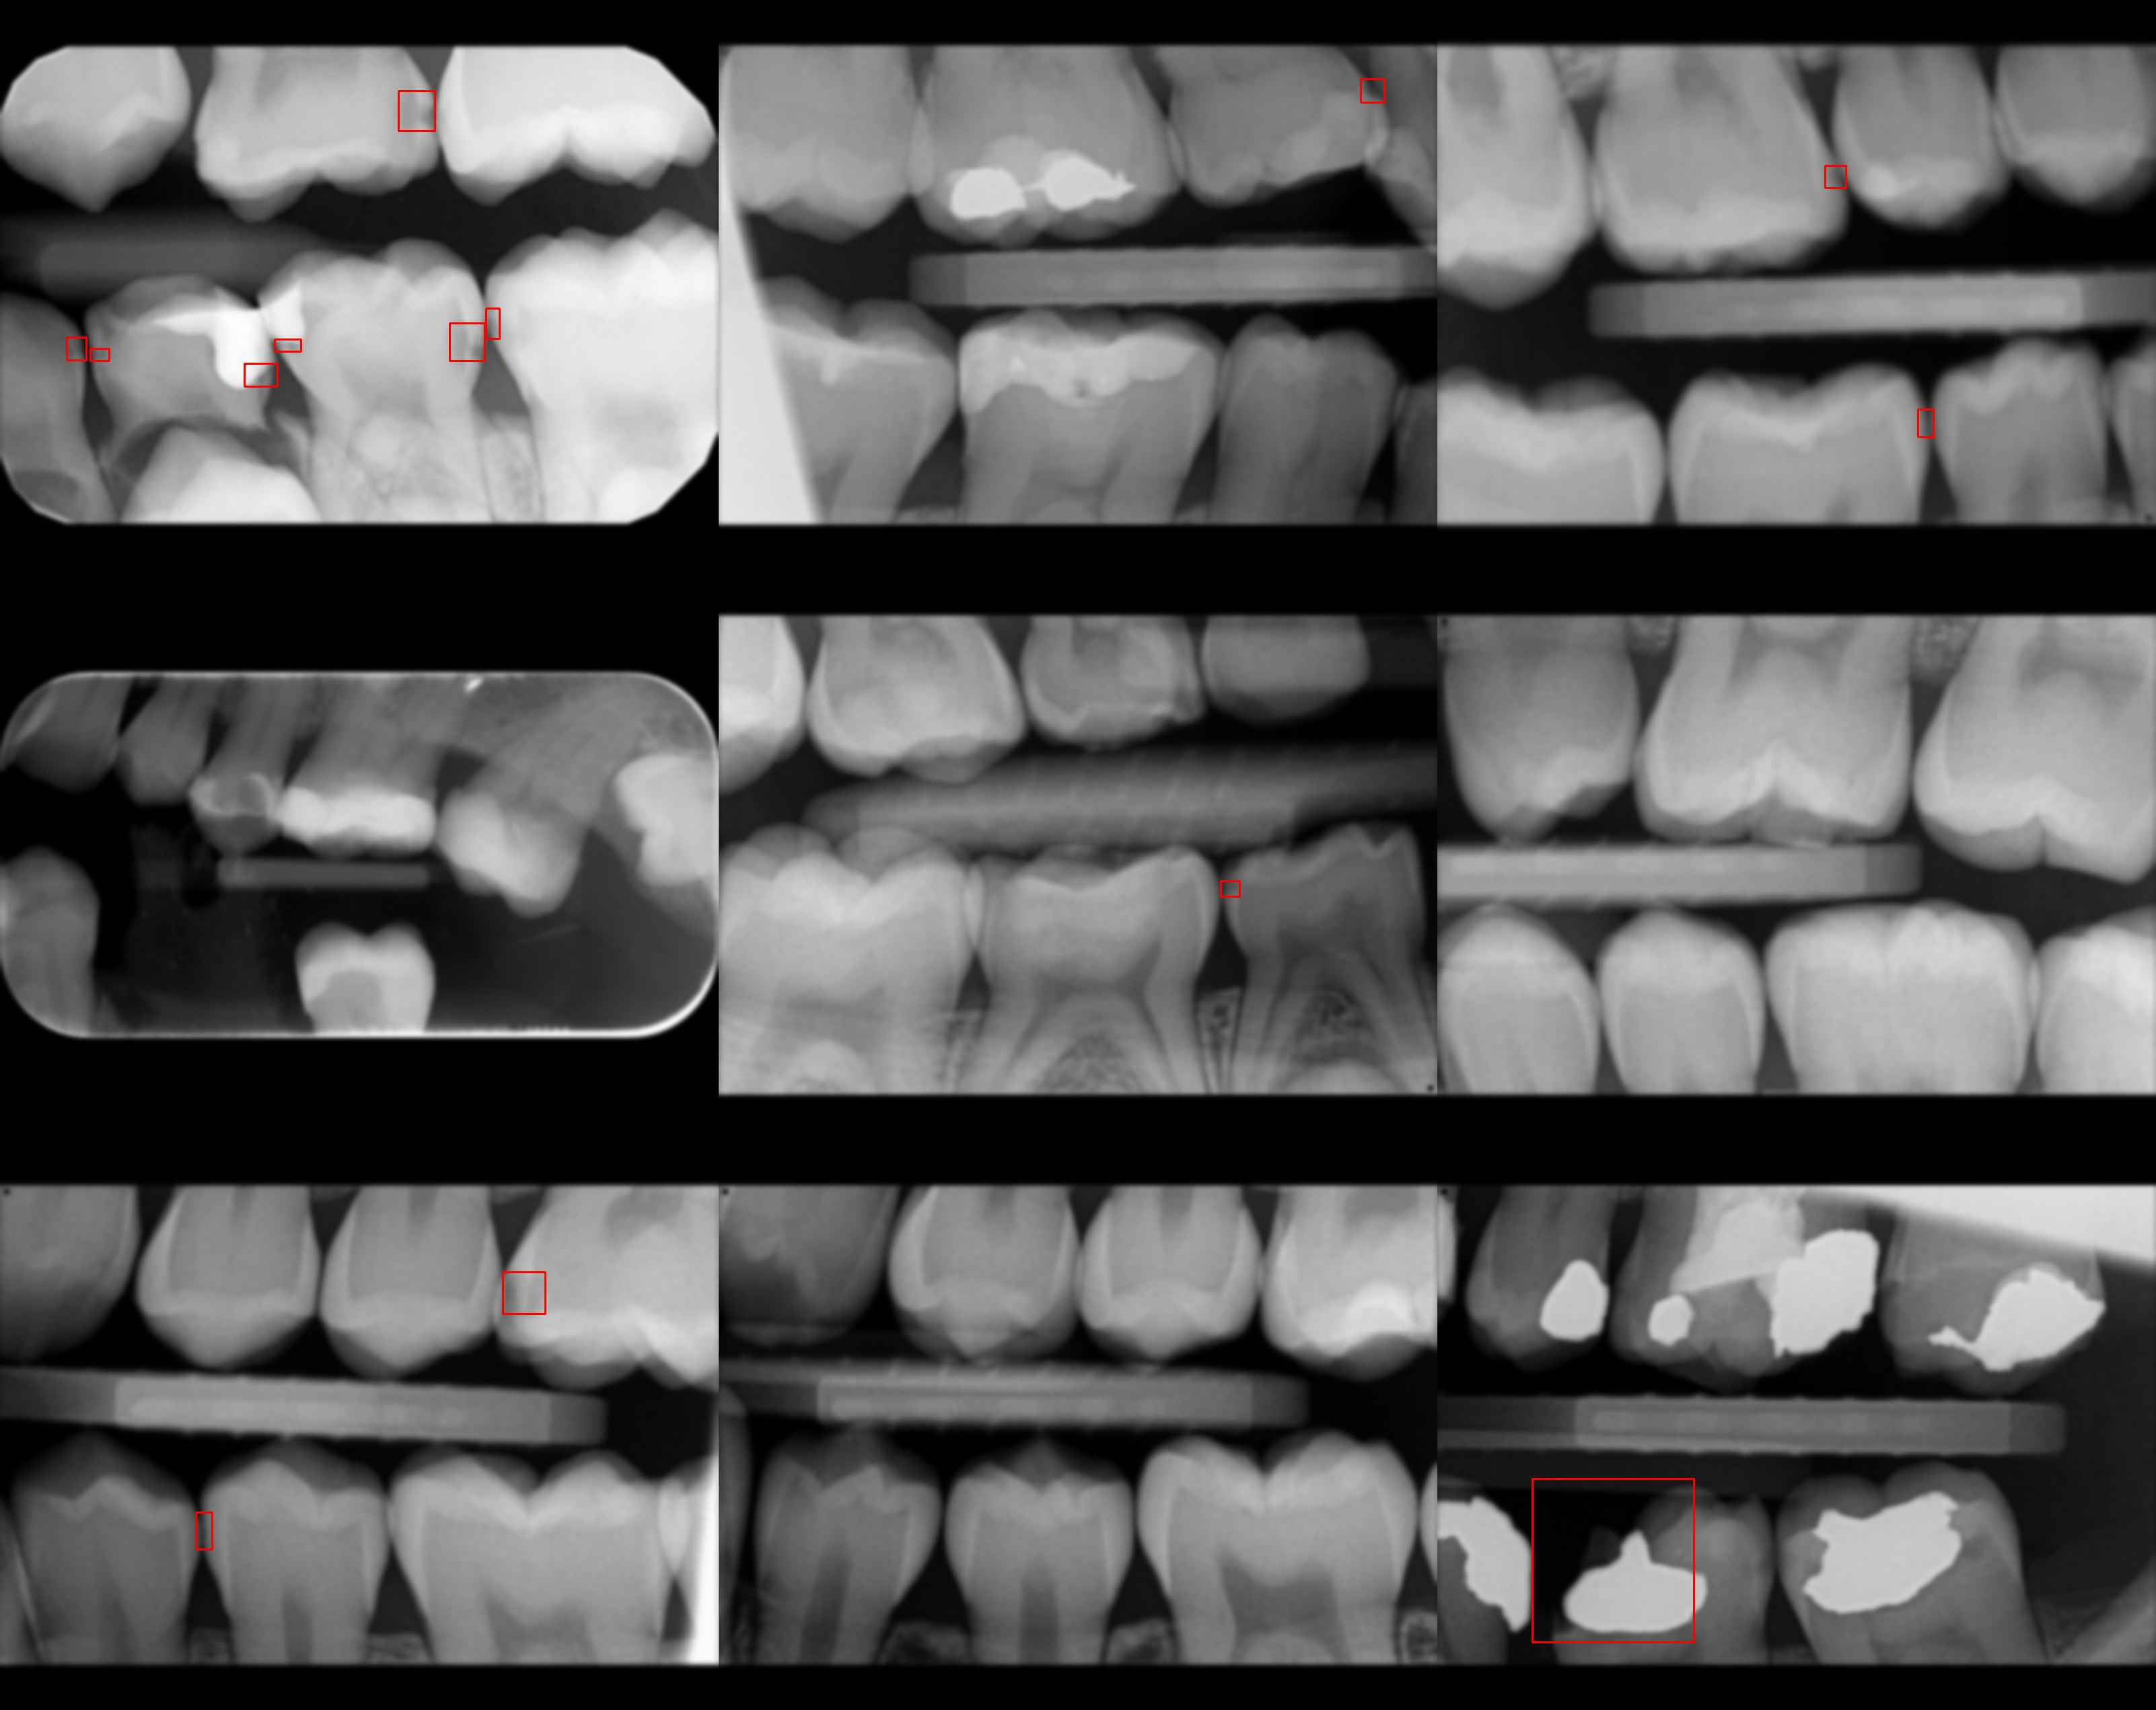
\includegraphics[width =0.9\linewidth]{images/gaussian_blur.jpg}
    \caption{Gaussian blur applied}
\end{figure}
\begin{figure}
    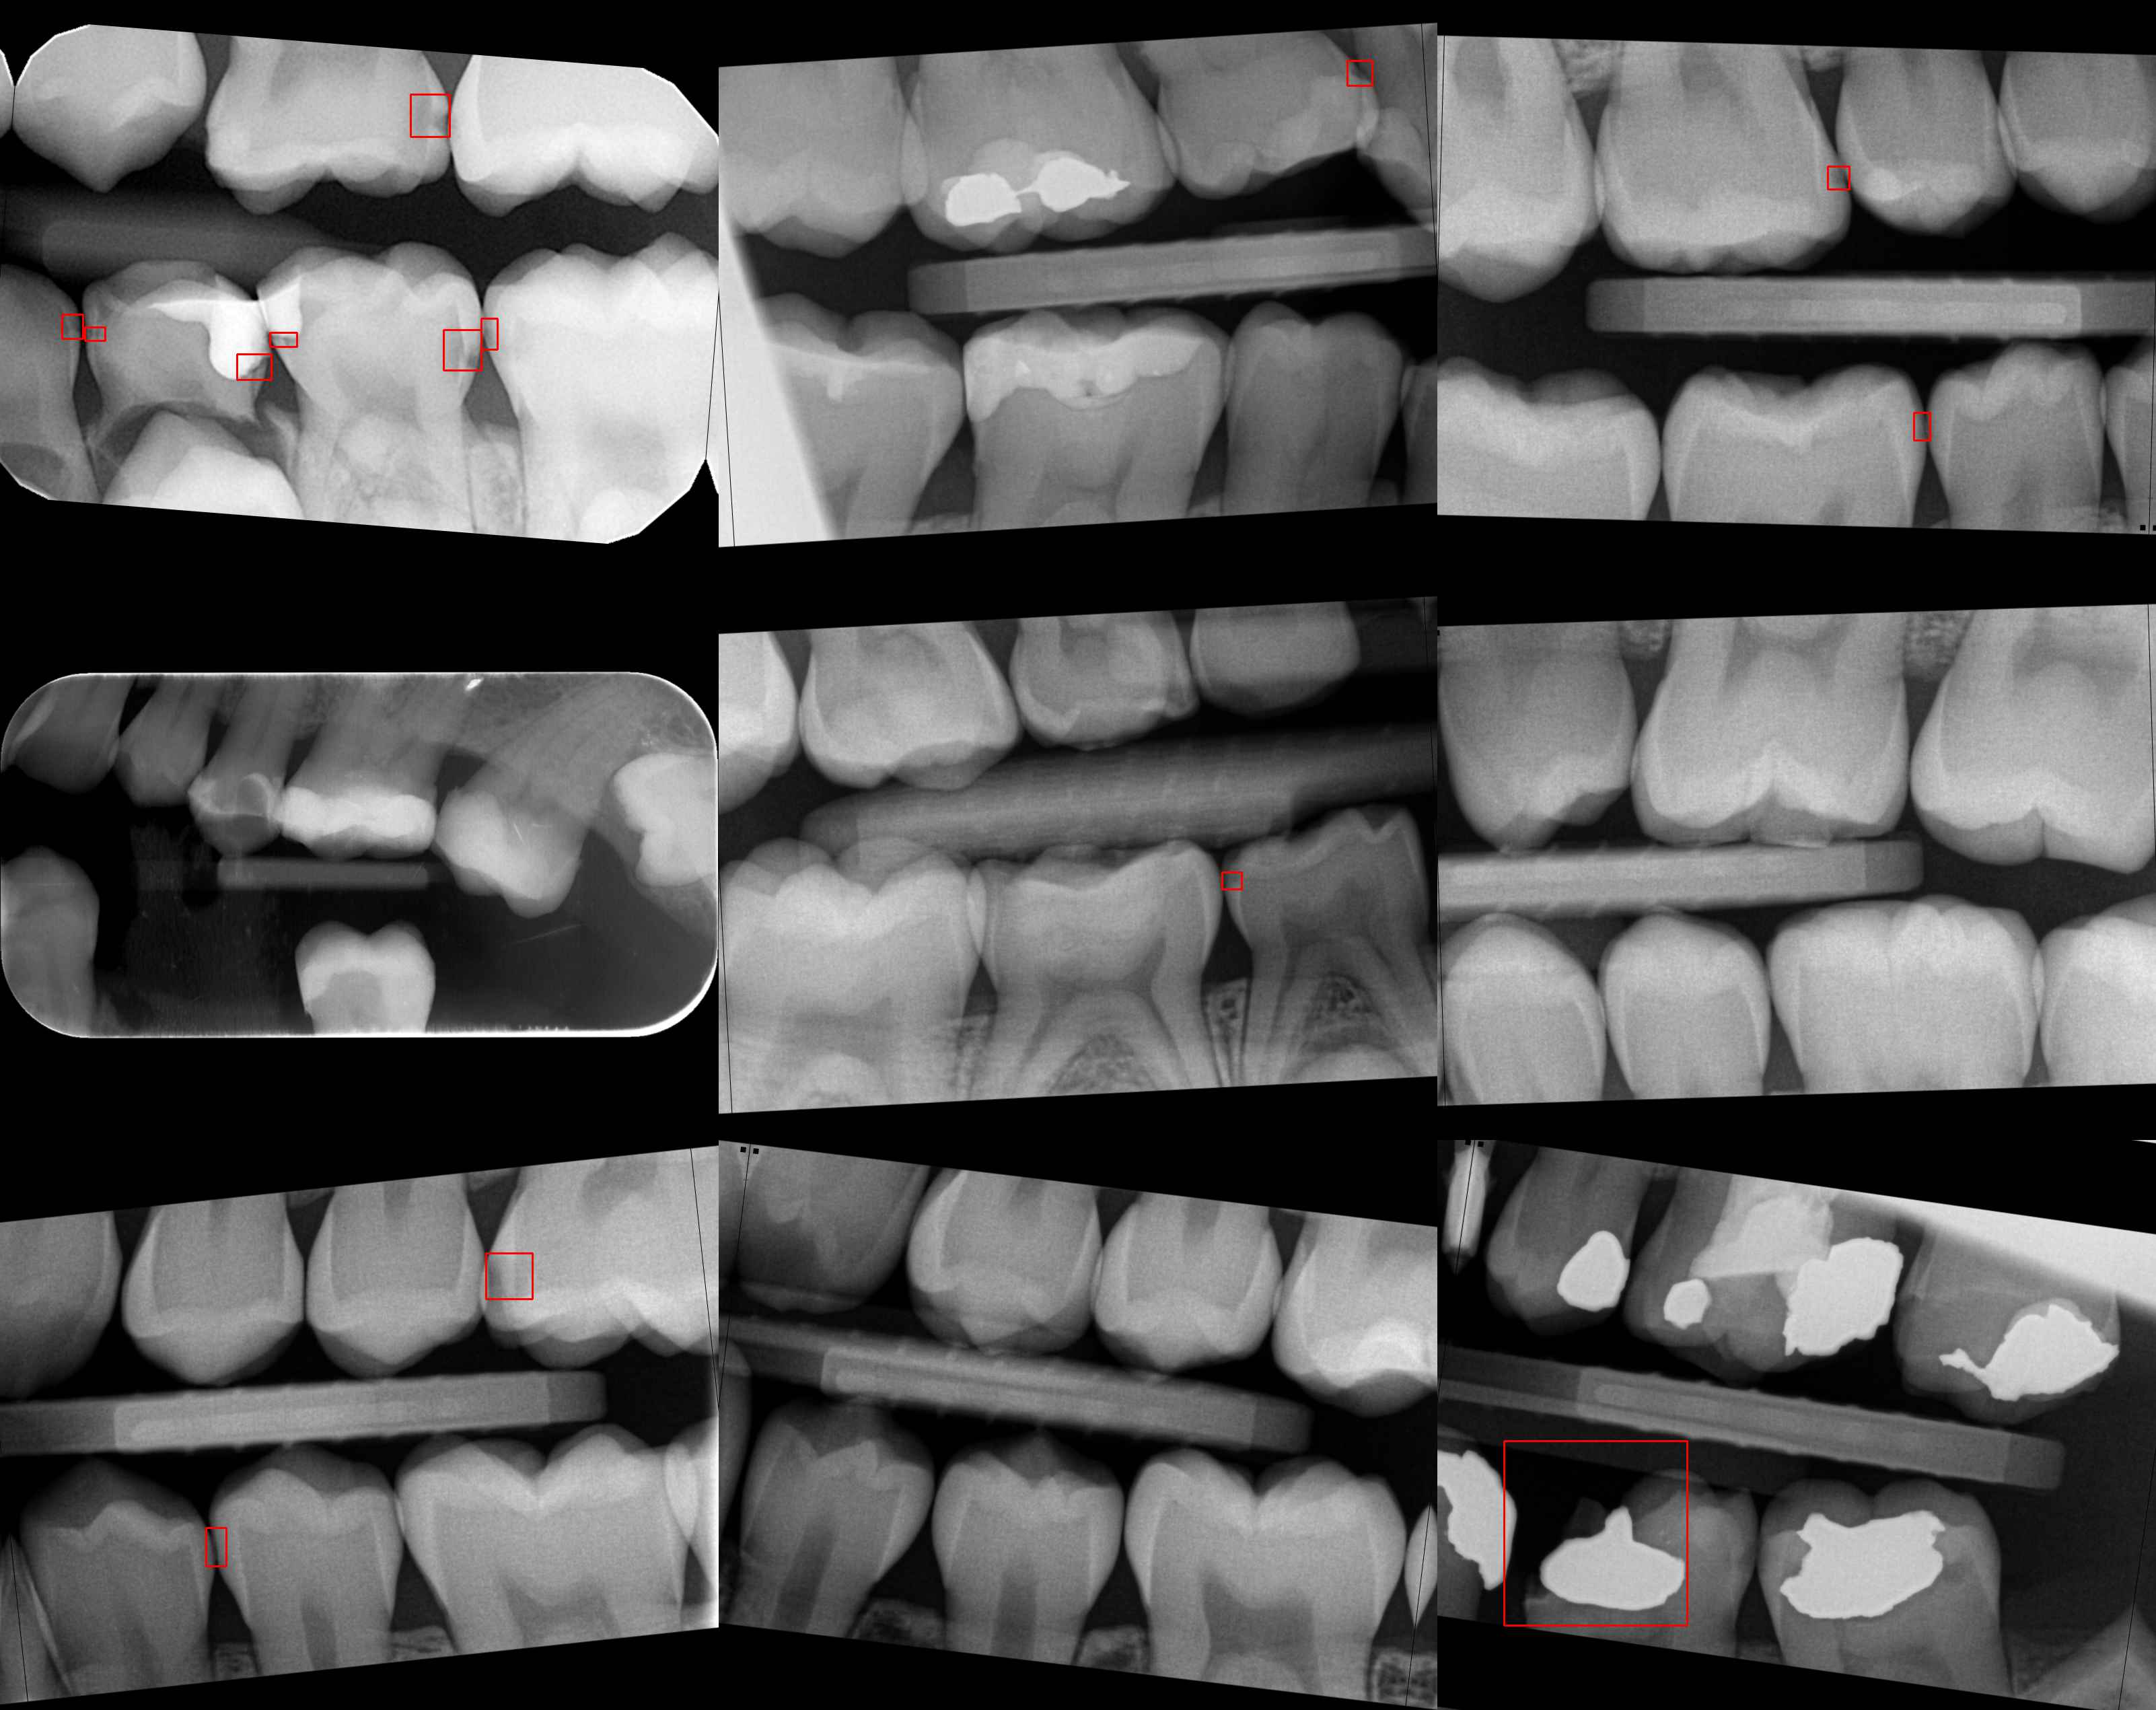
\includegraphics[width =0.9\linewidth]{images/roate_10.jpg}
    \caption{Rotation applied}
\end{figure}
\begin{figure}
    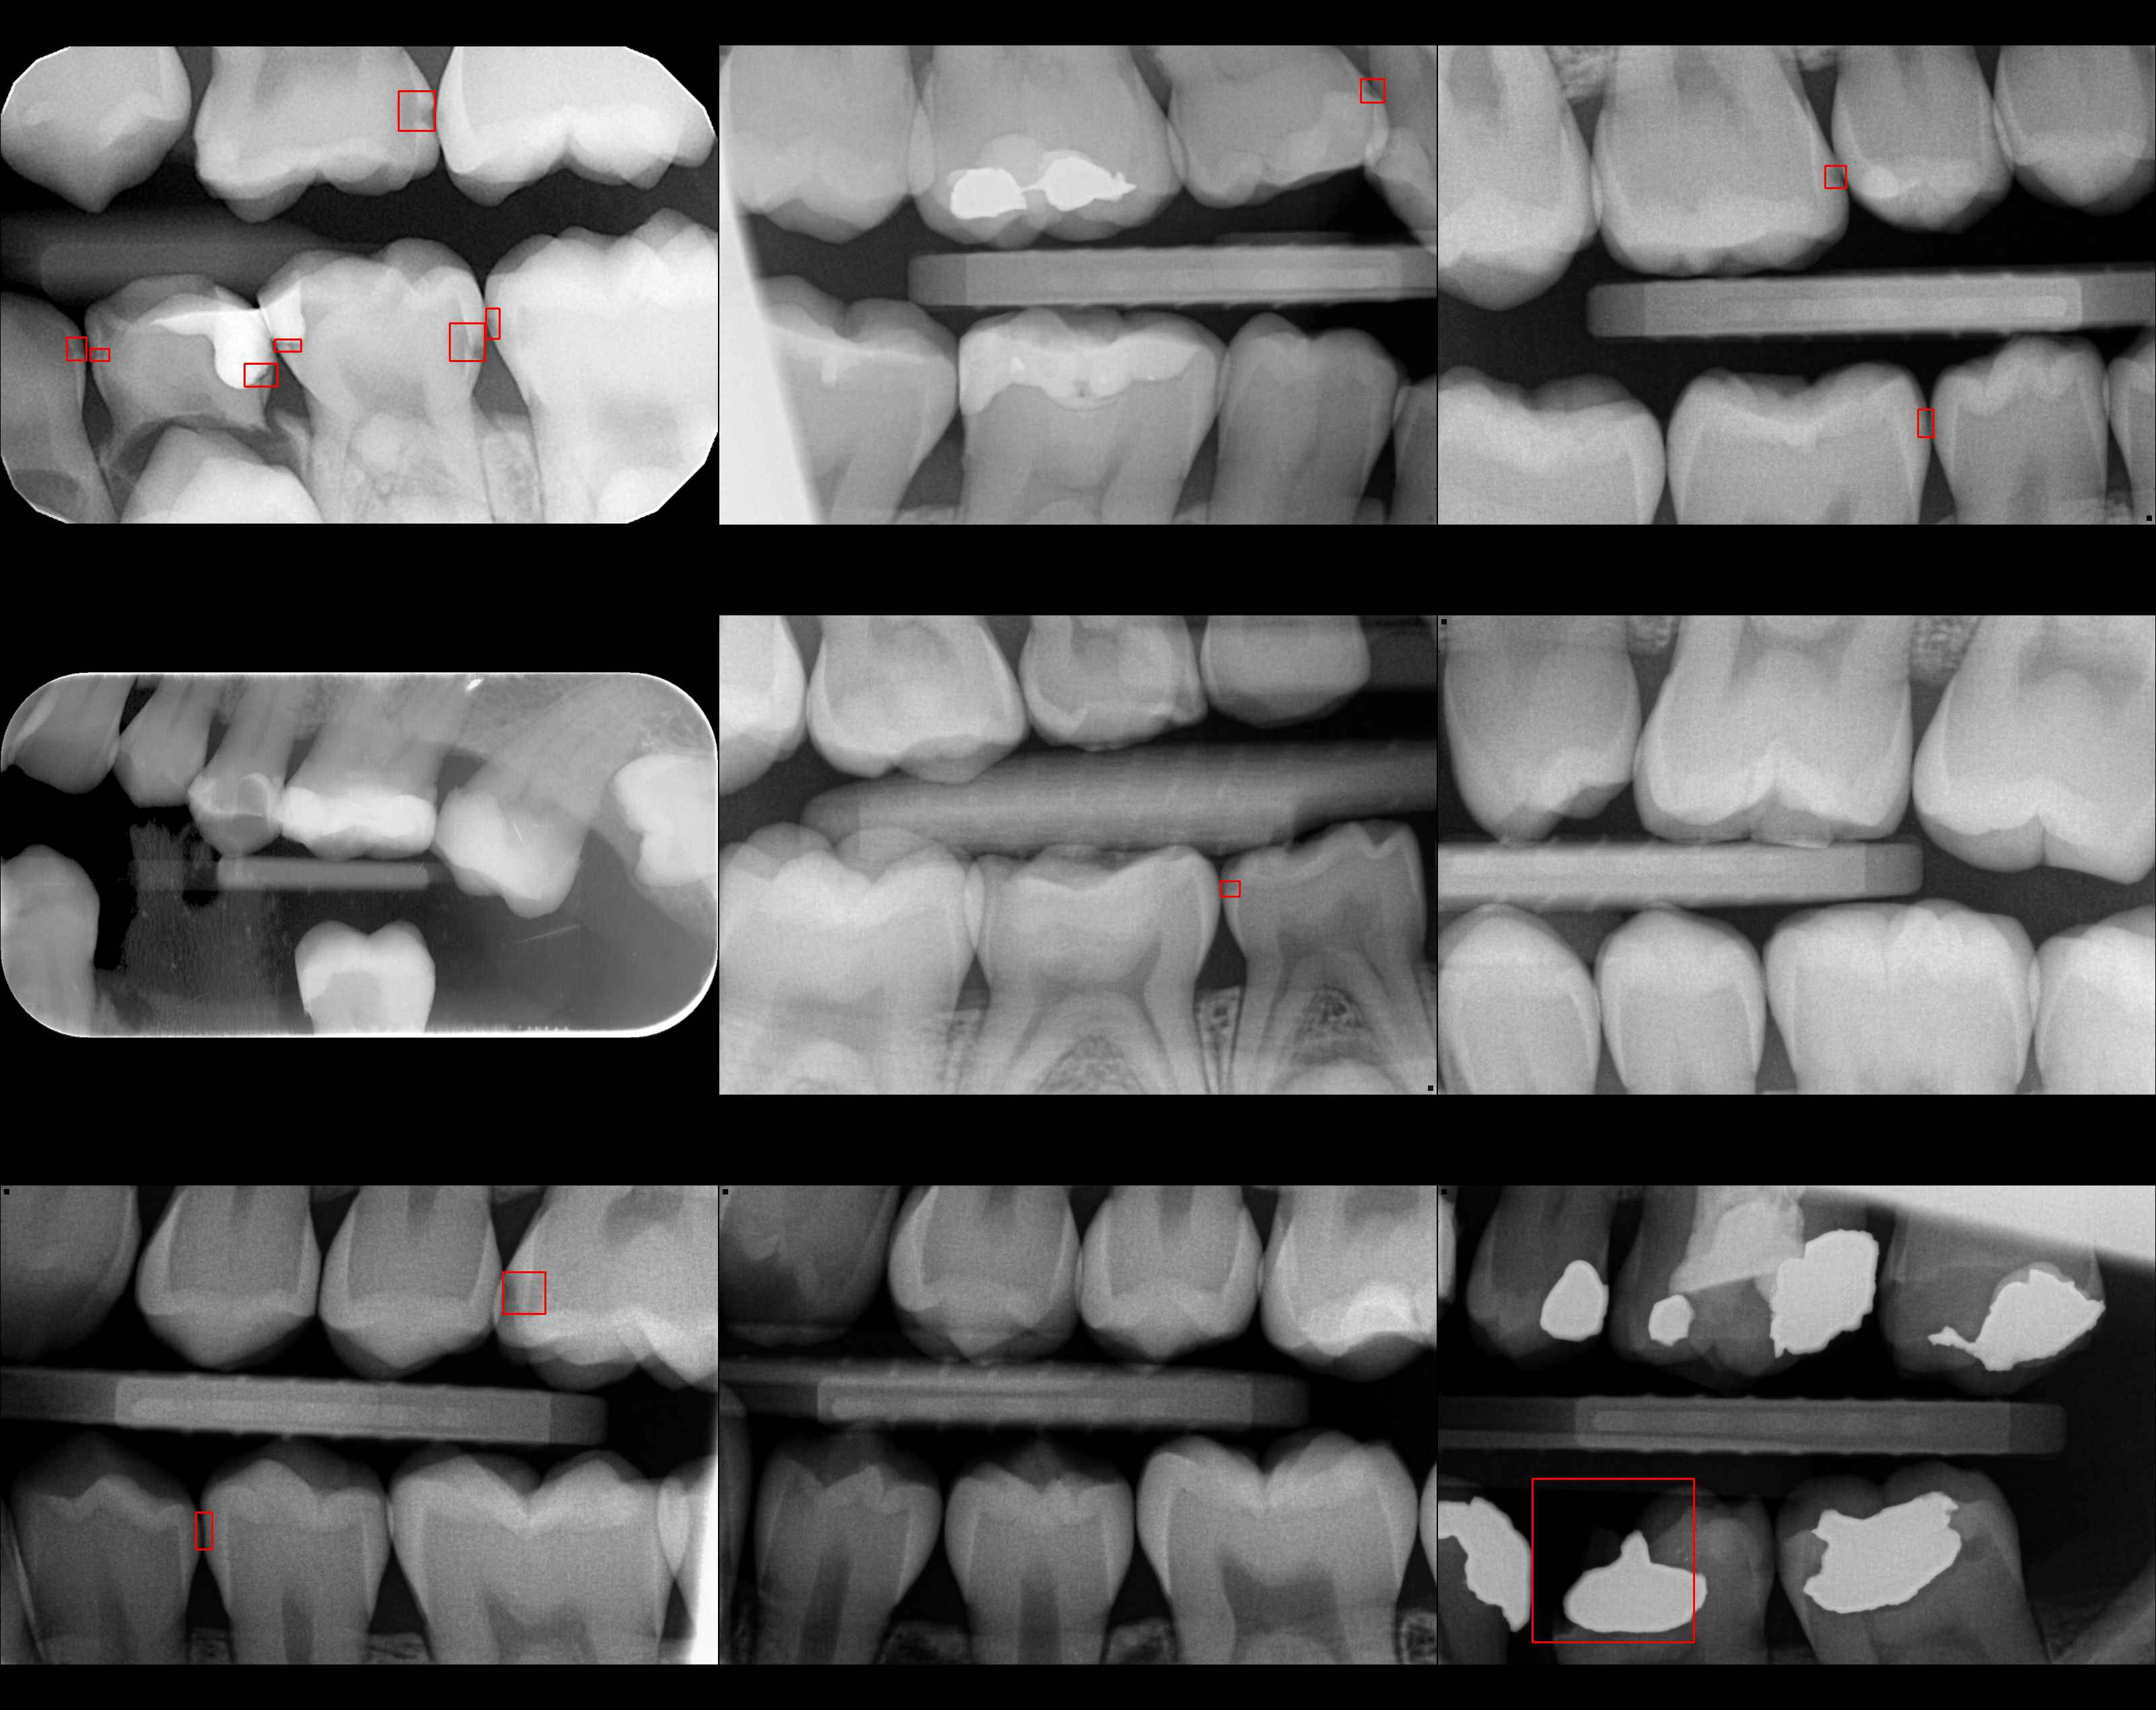
\includegraphics[width =0.9\linewidth]{images/random_gamma.jpg}
    \caption{Gamma correction applied}
\end{figure}
\begin{figure}
    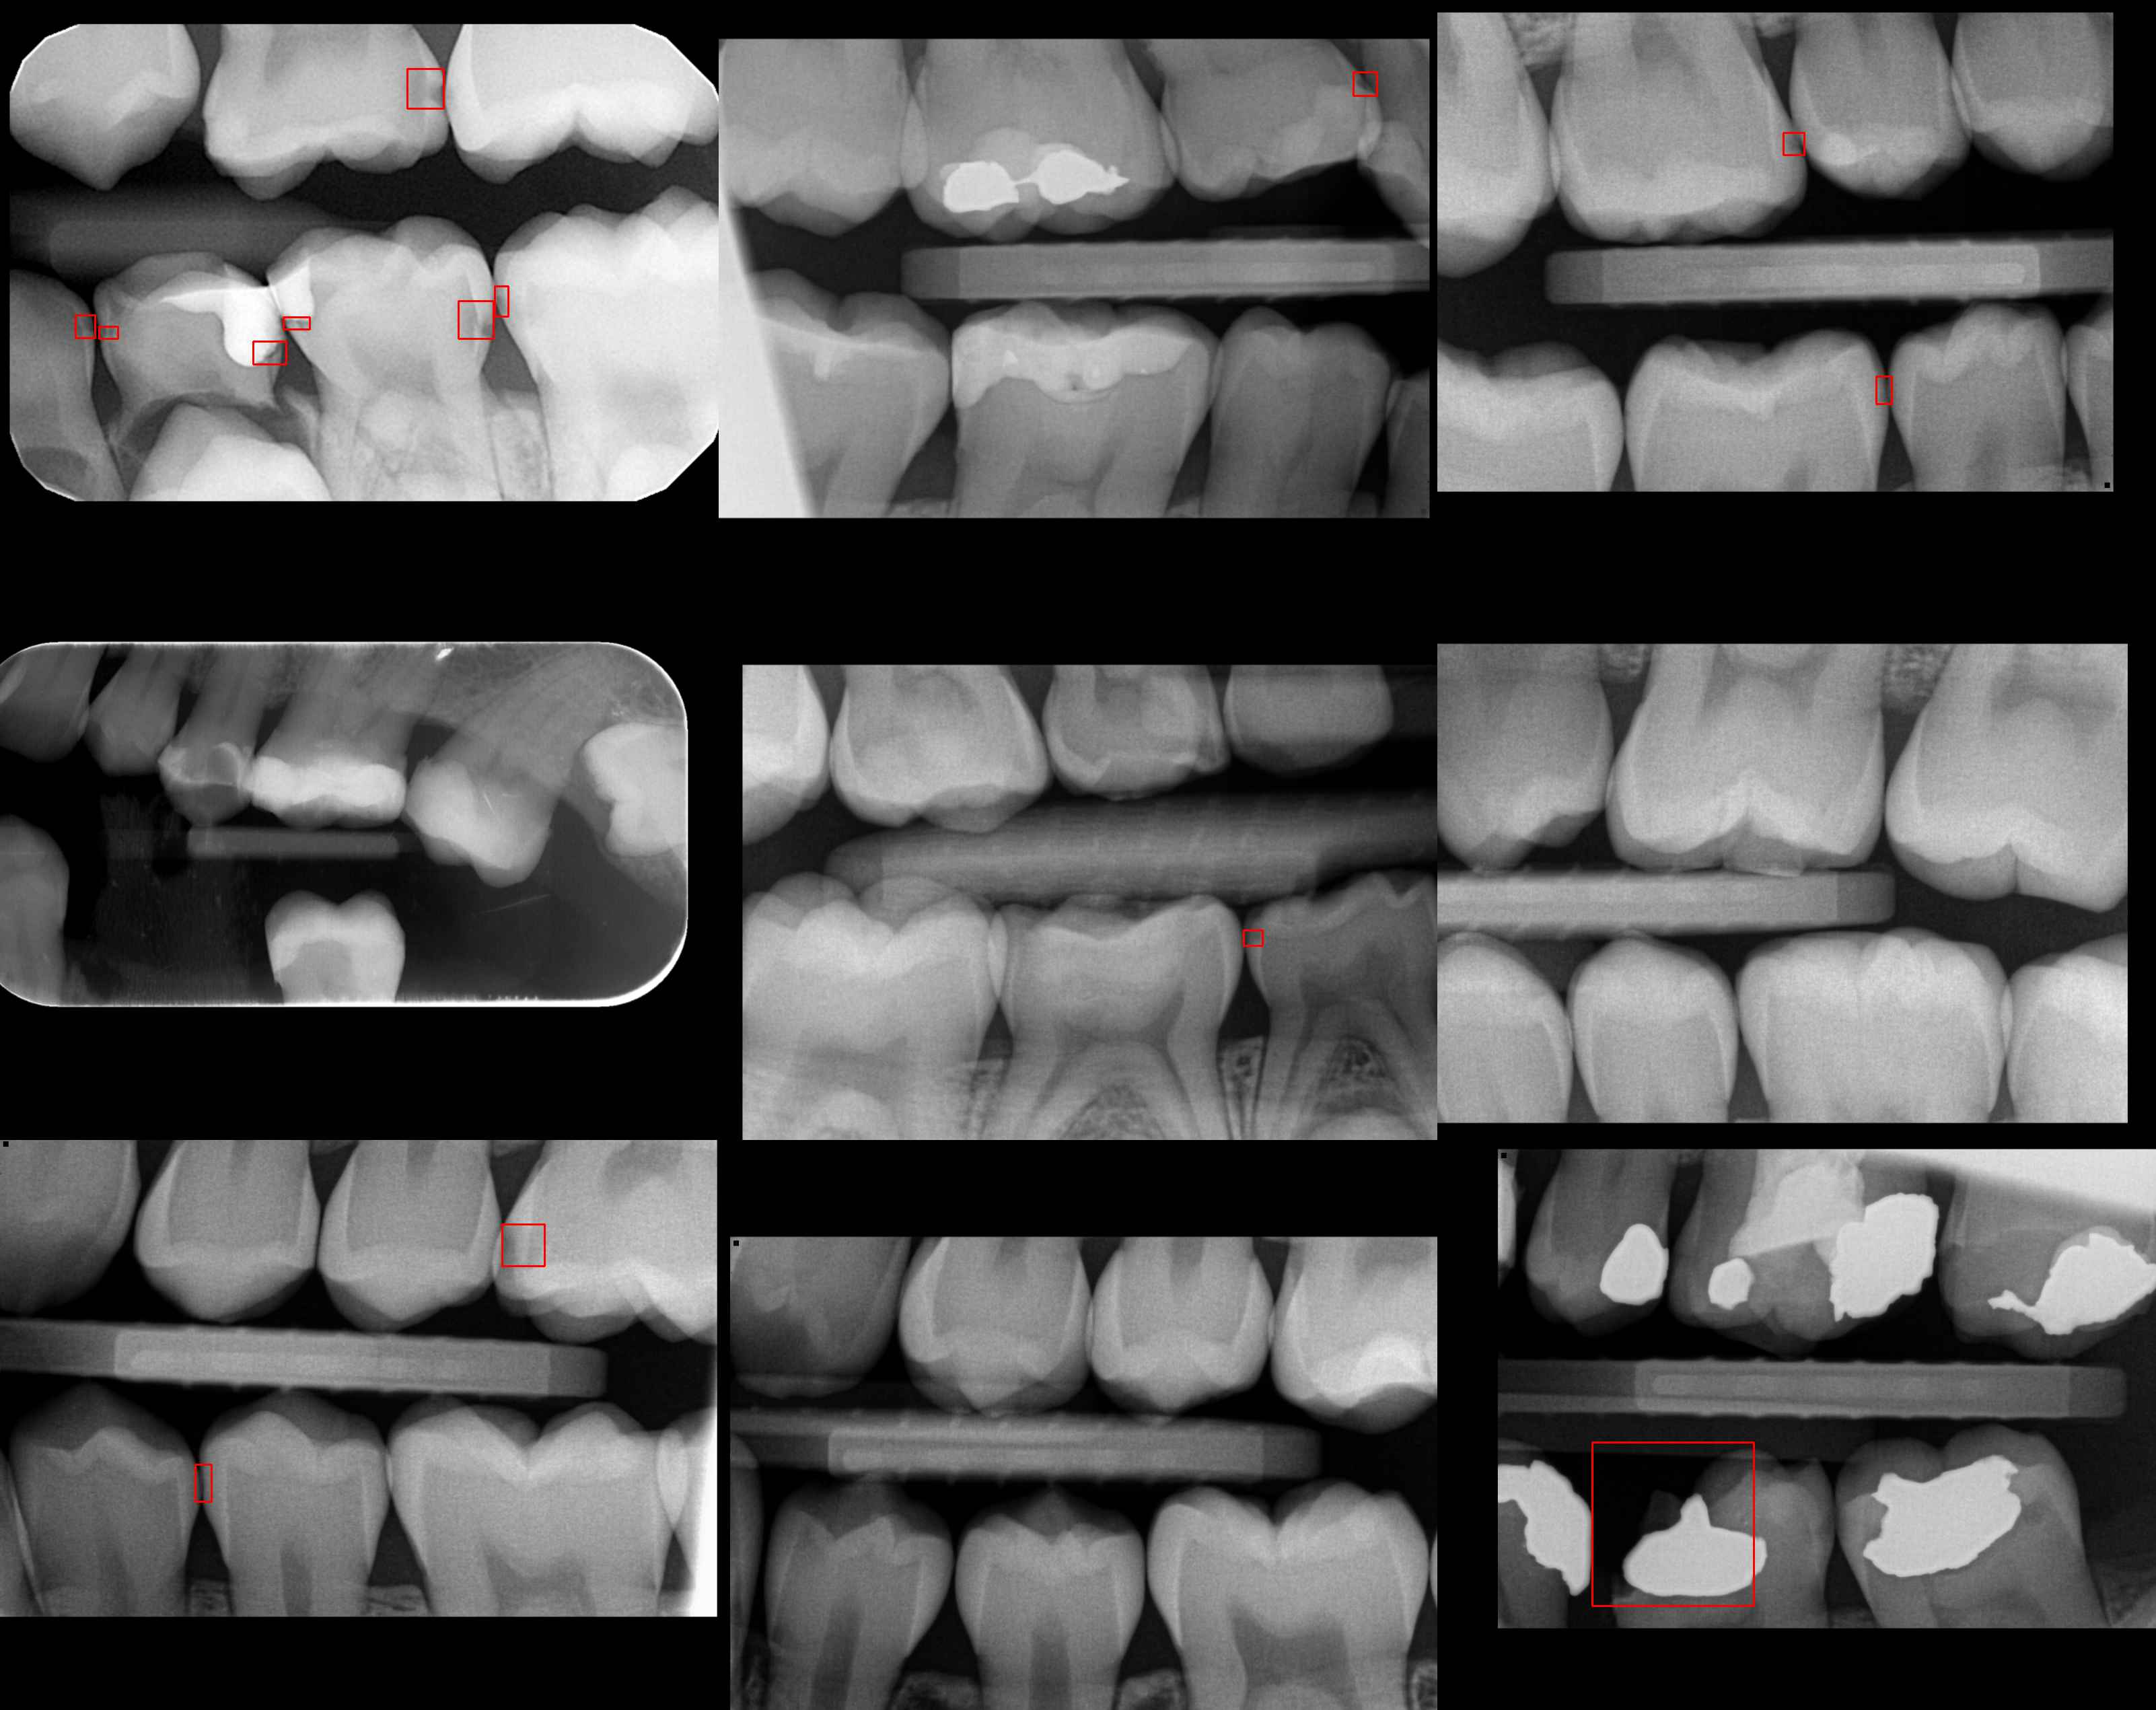
\includegraphics[width =0.9\linewidth]{images/translate.jpg}
    \caption{Translation applied}
\end{figure}
\begin{figure}
    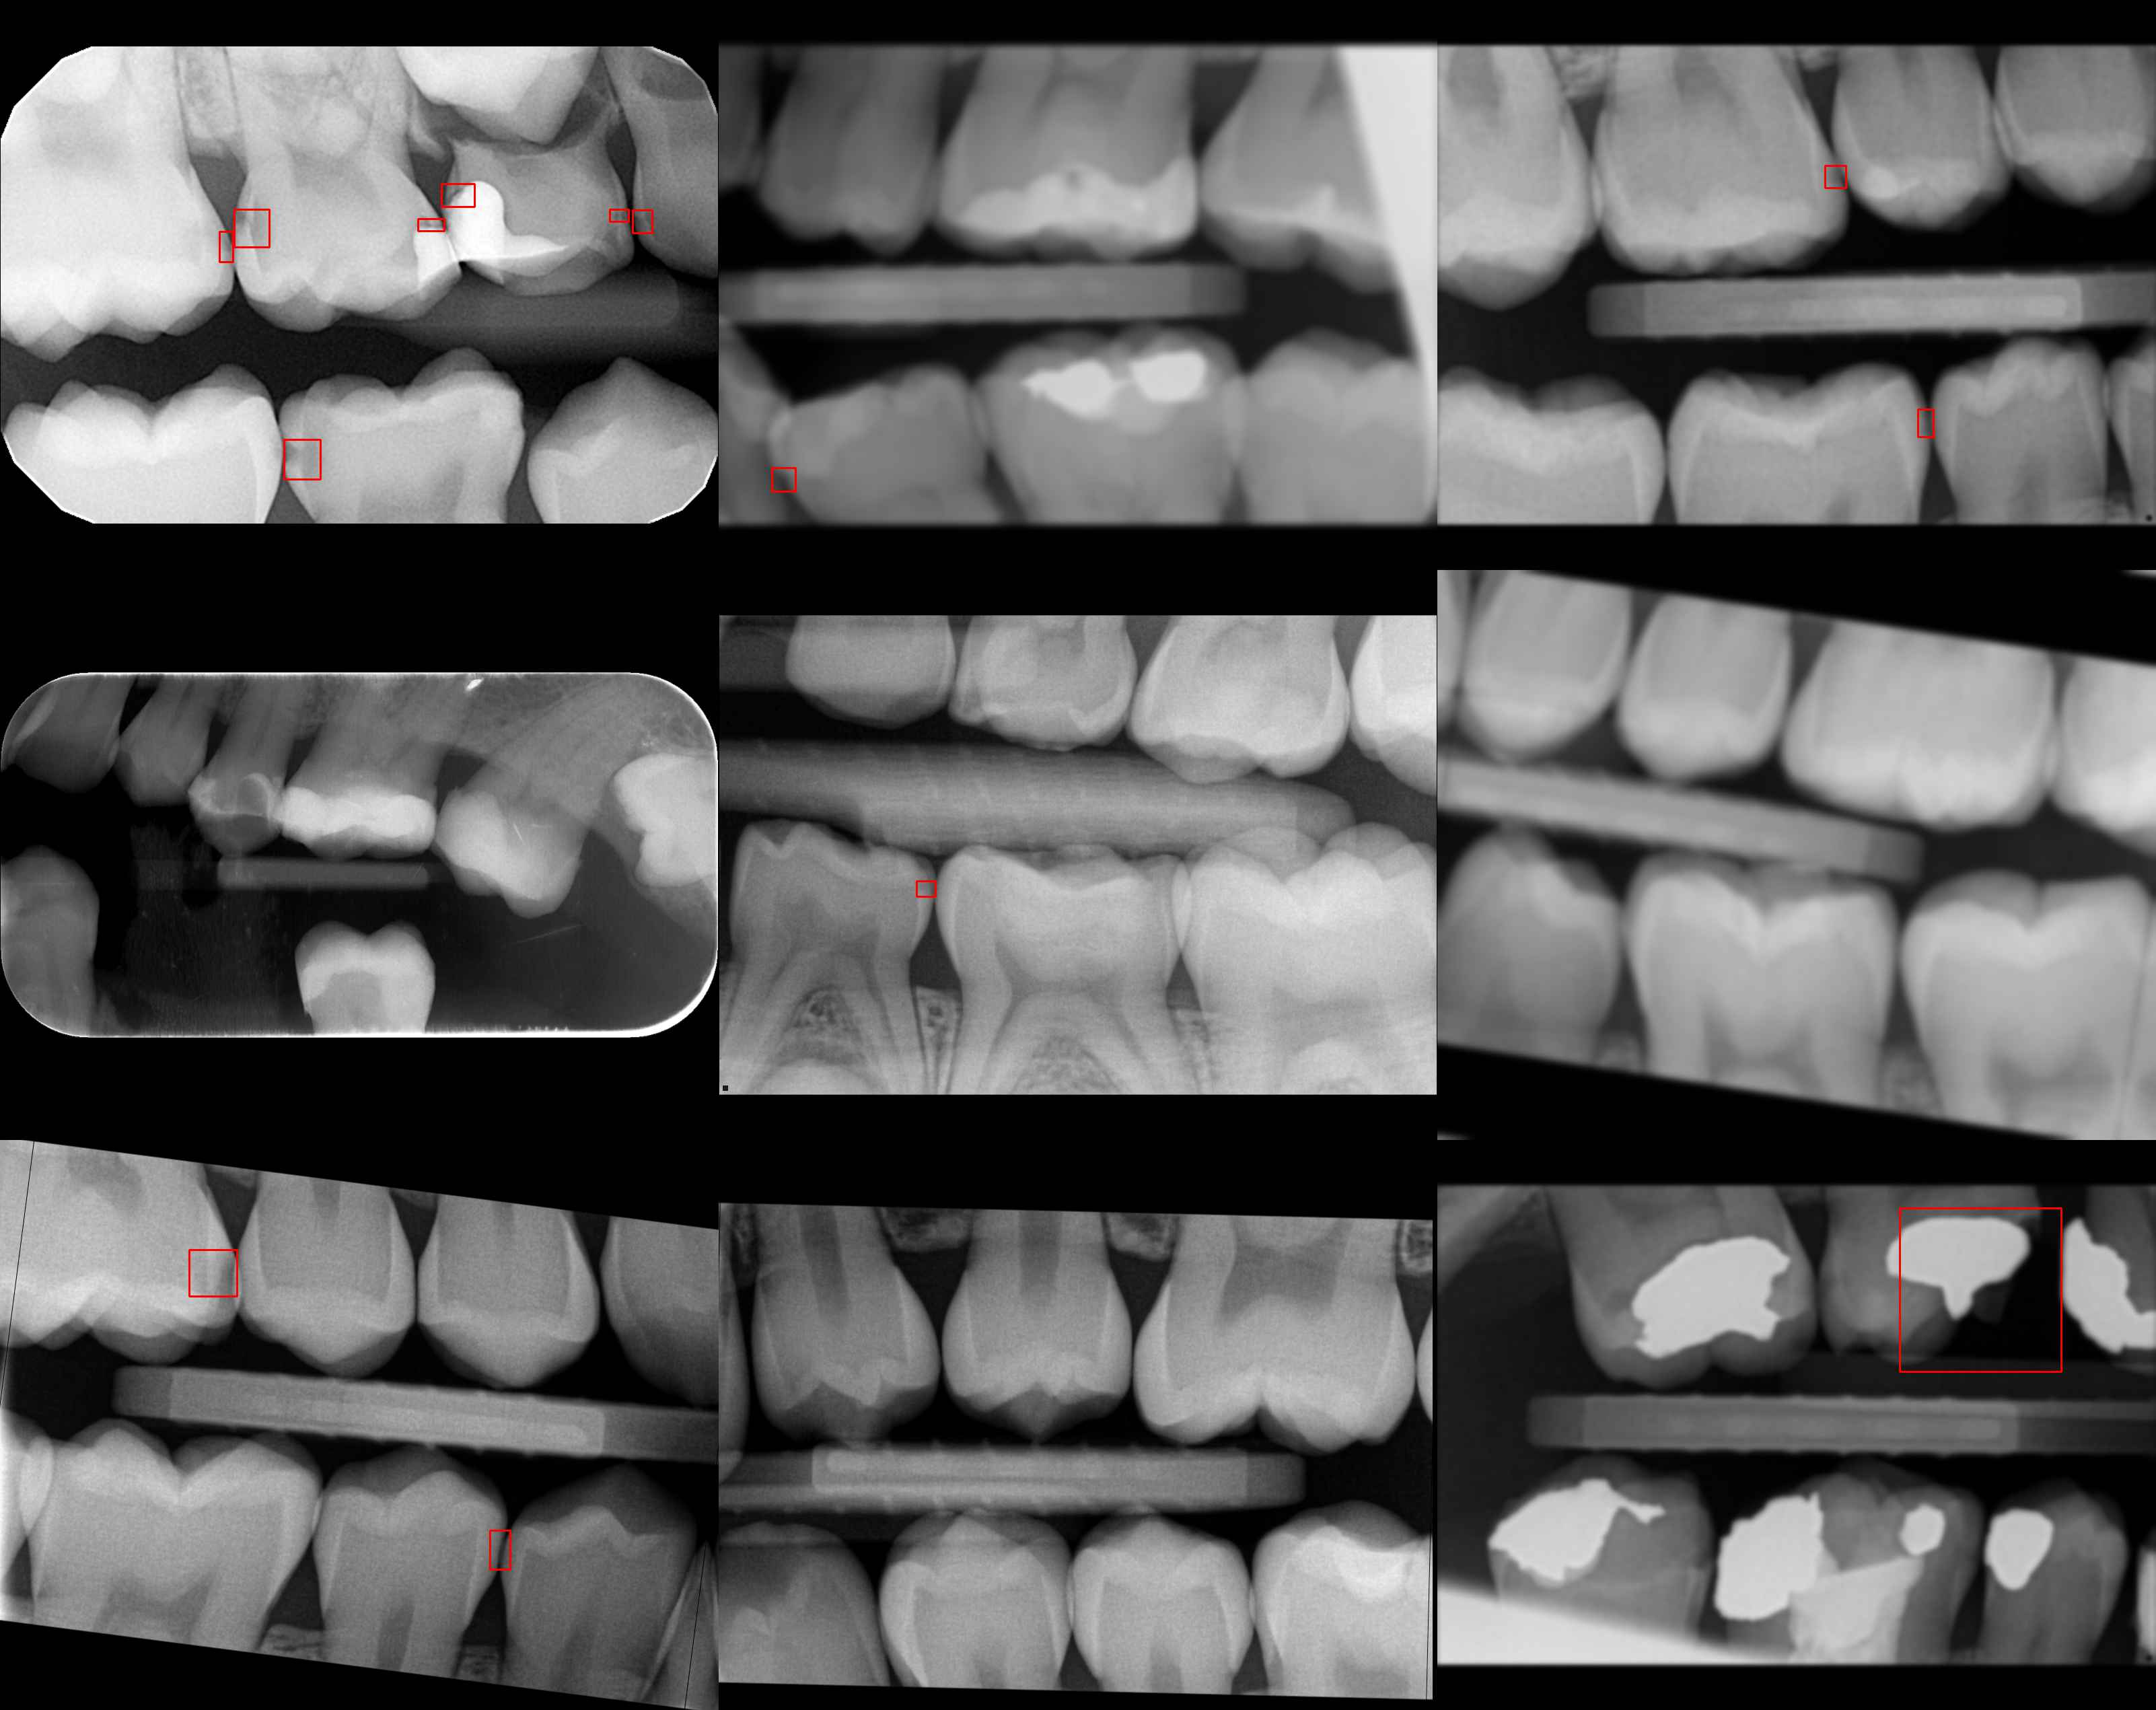
\includegraphics[width =0.9\linewidth]{images/all_transf.jpg}
    \caption{The whole augmentation pipeline applied}
\end{figure}

\end{document}
